\pdfoutput=1 % only if pdf/png/jpg images are used
%\documentclass[cits]{JINST}
\documentclass[a4paper,10pt]{scrartcl}
\usepackage{geometry}
\geometry{a4paper,left=26mm,right=26mm, top=2.2cm, bottom=3.4cm}

\usepackage{graphics}           % Unterstuetzung fuer Grafiken (extended)
\usepackage{graphicx}
\usepackage{subfigure}
\usepackage{amsmath}
\usepackage[amssymb]{SIunits}
%\usepackage[load-configurations=abbreviations,tight-spacing=true,separate-uncertainty,bracket-numbers = false]{siunitx} % JINST cannnot handle siunitx !!
\usepackage{nicefrac}
\usepackage[english]{babel}
\usepackage{lineno}
\usepackage{epstopdf}
\usepackage{stfloats}
\usepackage{upgreek}
\usepackage{verbatim}

\newcommand{\e}{\ensuremath{\mathnormal{e}}}
\newcommand{\h}{\ensuremath{\mathnormal{h}}}
\newcommand{\Datura}{\ensuremath{\mathnormal{DATURA}}}
\newcommand{\eV}{\ensuremath{\mathnormal{eV}}}

\setpagewiselinenumbers
\modulolinenumbers[5]
\linenumbers

\title{Status of the DATURA Telescope 2015}
\author{A. Author\thanks{Corresponding author: bla@bla.de}${}^{\,\,\,,\textrm{a}}$, B. Author${}^{\textrm{b}}$\\
${}^{\textrm{a}}$ Deutsches Elektronen-Synchrotron DESY, Hamburg, Germany,\\
${}^{\textrm{b}}$ Institute for Telescopocy, bla, blubb
}



% \abstract{
% The status of the $\Datura$ Telescope at DESY is summarised and the performance is shown with two example studies. 
% The pointing resolution using a 6\,GeV $\e$-beam at the centre of the telescope is $\unit{5}{\upmu\meter}$.
% }

%\keywords{Pixel, CMOS, Beam telescope, resolution, tracker} % need to be specified during submission


\begin{document}
\maketitle

Possible, possibly incomplete author list:\\
D. Eckstein\\
T. Eichhorn\\
H. Jansen\\
H. Perrey\\
R. Peschke\\
I. Rubinskiy\\
S. Spannagel\\
+ tbd w/ Ingrid

ToDo: Need to fix corresponding author


\abstract{
The status of the $\Datura$ Telescope at DESY is summarised and the performance is shown with two example studies. 
The pointing resolution using a 6\,GeV $\e$-beam at the centre of the telescope is $\unit{5}{\upmu\meter}$.
}

\tableofcontents
\newpage



\section{Introduction}
\label{sec:intro}

Beam telescopes are vital tools for R\&D projects focussing on position sensitive particle detection sensors. 
These range from collider-specific detectors with high radiation tolerance~\cite{1748-0221-9-12-C12001,1748-0221-9-12-C12029},
 high resolution and low material requirements~\cite{1748-0221-10-03-C03044} to medical applications~\cite{Ballabriga2011S15}, among others. 
Complementary to sensor simulations using finite element analysis tools, test beam studies are used at various stages of sensor and read-out chip development. 
%Also in future high-energy physics experiments pixel detectors will be used in the inner layers of the tracking devices. 
%The demands are challenging and range from high speed and high radiation-hardness for the high-luminosity LHC (HL-LHC)
% experiments\,\cite{Nurnberg:2014aya, Garcia-Argos:2015zda} to high resolution and low mass at the International Linear Collider (ILC)\,\cite{ILC} or at the Compact Linear Collider (CLIC)\,\cite{CLIC}. 
Such test beam studies are well suited and often used for the evaluation of the performance of a detector prototype. % developed within the various R\&D projects. 

Within the Integrated Infrastructure Initiative funded by the EU in the 6th framework programme,
 the EUDET project aimed at providing a high-resolution pixel beam telescope for test beam studies~\cite{ref:eudetreport200902}.
%In order to carry out these measurements a high-resolution pixel beam telescope was developed within the $\eudet$ project~\cite{ref:eudetreport200902},
The guidelines for the development were to allow for an easy integration of custom data acquisition systems covering a wide range of readout schemes, latencies, and acquisition rates.
This is achieved by well defined interfaces on both the hardware and the software level. 
Fast LHC-type tracking devices are integrable in the same manner as slower rolling-shutter readout devices. 

A EUDET-type beam telescope consists of six pixel detector planes equipped with fine-pitch $\Mimosa$ sensors~\cite{HuGuo2010480},
 the mechanics for precise positioning of the device under test (DUT) and the telescope planes in the beam, a Trigger Logic Unit (TLU) providing trigger capabilities and a data acquisition system.
The chosen design meets most user requirements in terms of easy integration capabilities, spatial resolution, and trigger rates. 
The telescope planes are designed and built to keep the material budget as low as possible in order to achieve an excellent track resolution
 even at the rather low particle energies of up to 6\,GeV at the DESY test beam facilities.

The original EUDET beam telescope, which was modified to become the AIDA telescope, is operated at SPS beamline H6 (CERN).
Responding to the increasing demand of the sensor R\&D community, several replicas, collectively called $\eudet$-type beam telescopes, have been built since then:
 ACONITE for the ATLAS group, which is also operated at the beamline H6, ANEMONE at ELSA (University of Bonn), the copy for the Carlton University called CALADIUM, 
 and two copies, $\Datura$ and DURANTA, which are operated at DESY. 
 Within the AIDA2020 project, another copy is going to be built -- operation is foreseen at the PS beamline (CERN).
All replicas are based on the $\Mimosa$ sensors and are equipped with the same data acquisition system and software framework. 
The EUDET telescope has been used since 2007 in various stages of development by hundreds of users and played an important role in sensor studies employed by a wide community. 
From January 2013 until March 2014 alone, about 300 users utilised an $\eudet$-type beam telescope at DESY for a total of 80 user weeks. 
The results reported here are based on data taken with $\Datura$ at test beam area~21 at {DESY-II} and are comparable to other beam telescope copies with
a similar thickness of the epitaxial layer~\cite{desy-tscopes-main}. 

This paper is organised as follows: 
The DESY beamlines are introduced in section~\ref{sec:beamlines}, followed by the description of the beam telescope
 and the data acquisition framework in sections~\ref{sec:tscope} and~\ref{sec:eudaq}, respectively.
Section~\ref{sec:offline} details the offline analysis and reconstruction software. 
Results of the EUDET-type beam telescope performance and track resolution predictions for different telescope configurations and beam momenta are presented in section~\ref{sec:trackres}. 
Additionally, the prediction of the standard deviation of the angular scattering distributions is compared to measurements with an electron beam. 
%The measured data is complemented by analytic predictions using the formalism of General Broken Lines (GBL)~\cite{Blobel20111760,Kleinwort-2012}.
Section~\ref{sec:dutintegration} discusses the integration of DUTs into an $\eudet$-type beam telescope. 
%With these GBL predictions at hand, the optimal telescope geometry can be calculated for a given set-up (DUT, cooling, ...) prior to the test beam.


\section{Beamlines}
\label{sec:beamlines}

\subsection{DESY-II}

qwert

\subsection{SPS}

qwerty

\section{The DATURA telescope}
\label{sec:aida}

The DESY-type beam telescope are tabletop tracking detectors featuring six pixelated silicon sensors, four scintillators with photo multiplier tubes (PMTs) for trigger purposes,
 a Trigger Logic Unit (TLU) providing trigger logic and time stamp information on particle passage, and a data acquisition system for the data readout. 
Figure\,\ref{fig:datura-tscope} shows the beam telescope with its sensor jigs, wherein the pixel sensors are embedded, with its auxiliary boards providing connections for power,
 sensor configuration, clock signals, and data transmission. 
The planes are organised in two telescope arms holding three sensors each. 
A DUT can be inserted between the arms or at either end of the beam telescope. 
In the Cartesian, right-handed coordinate system chosen, the $x$-direction points horizontally and $z$-direction along the beam.

\begin{figure}[tb]
	\center
	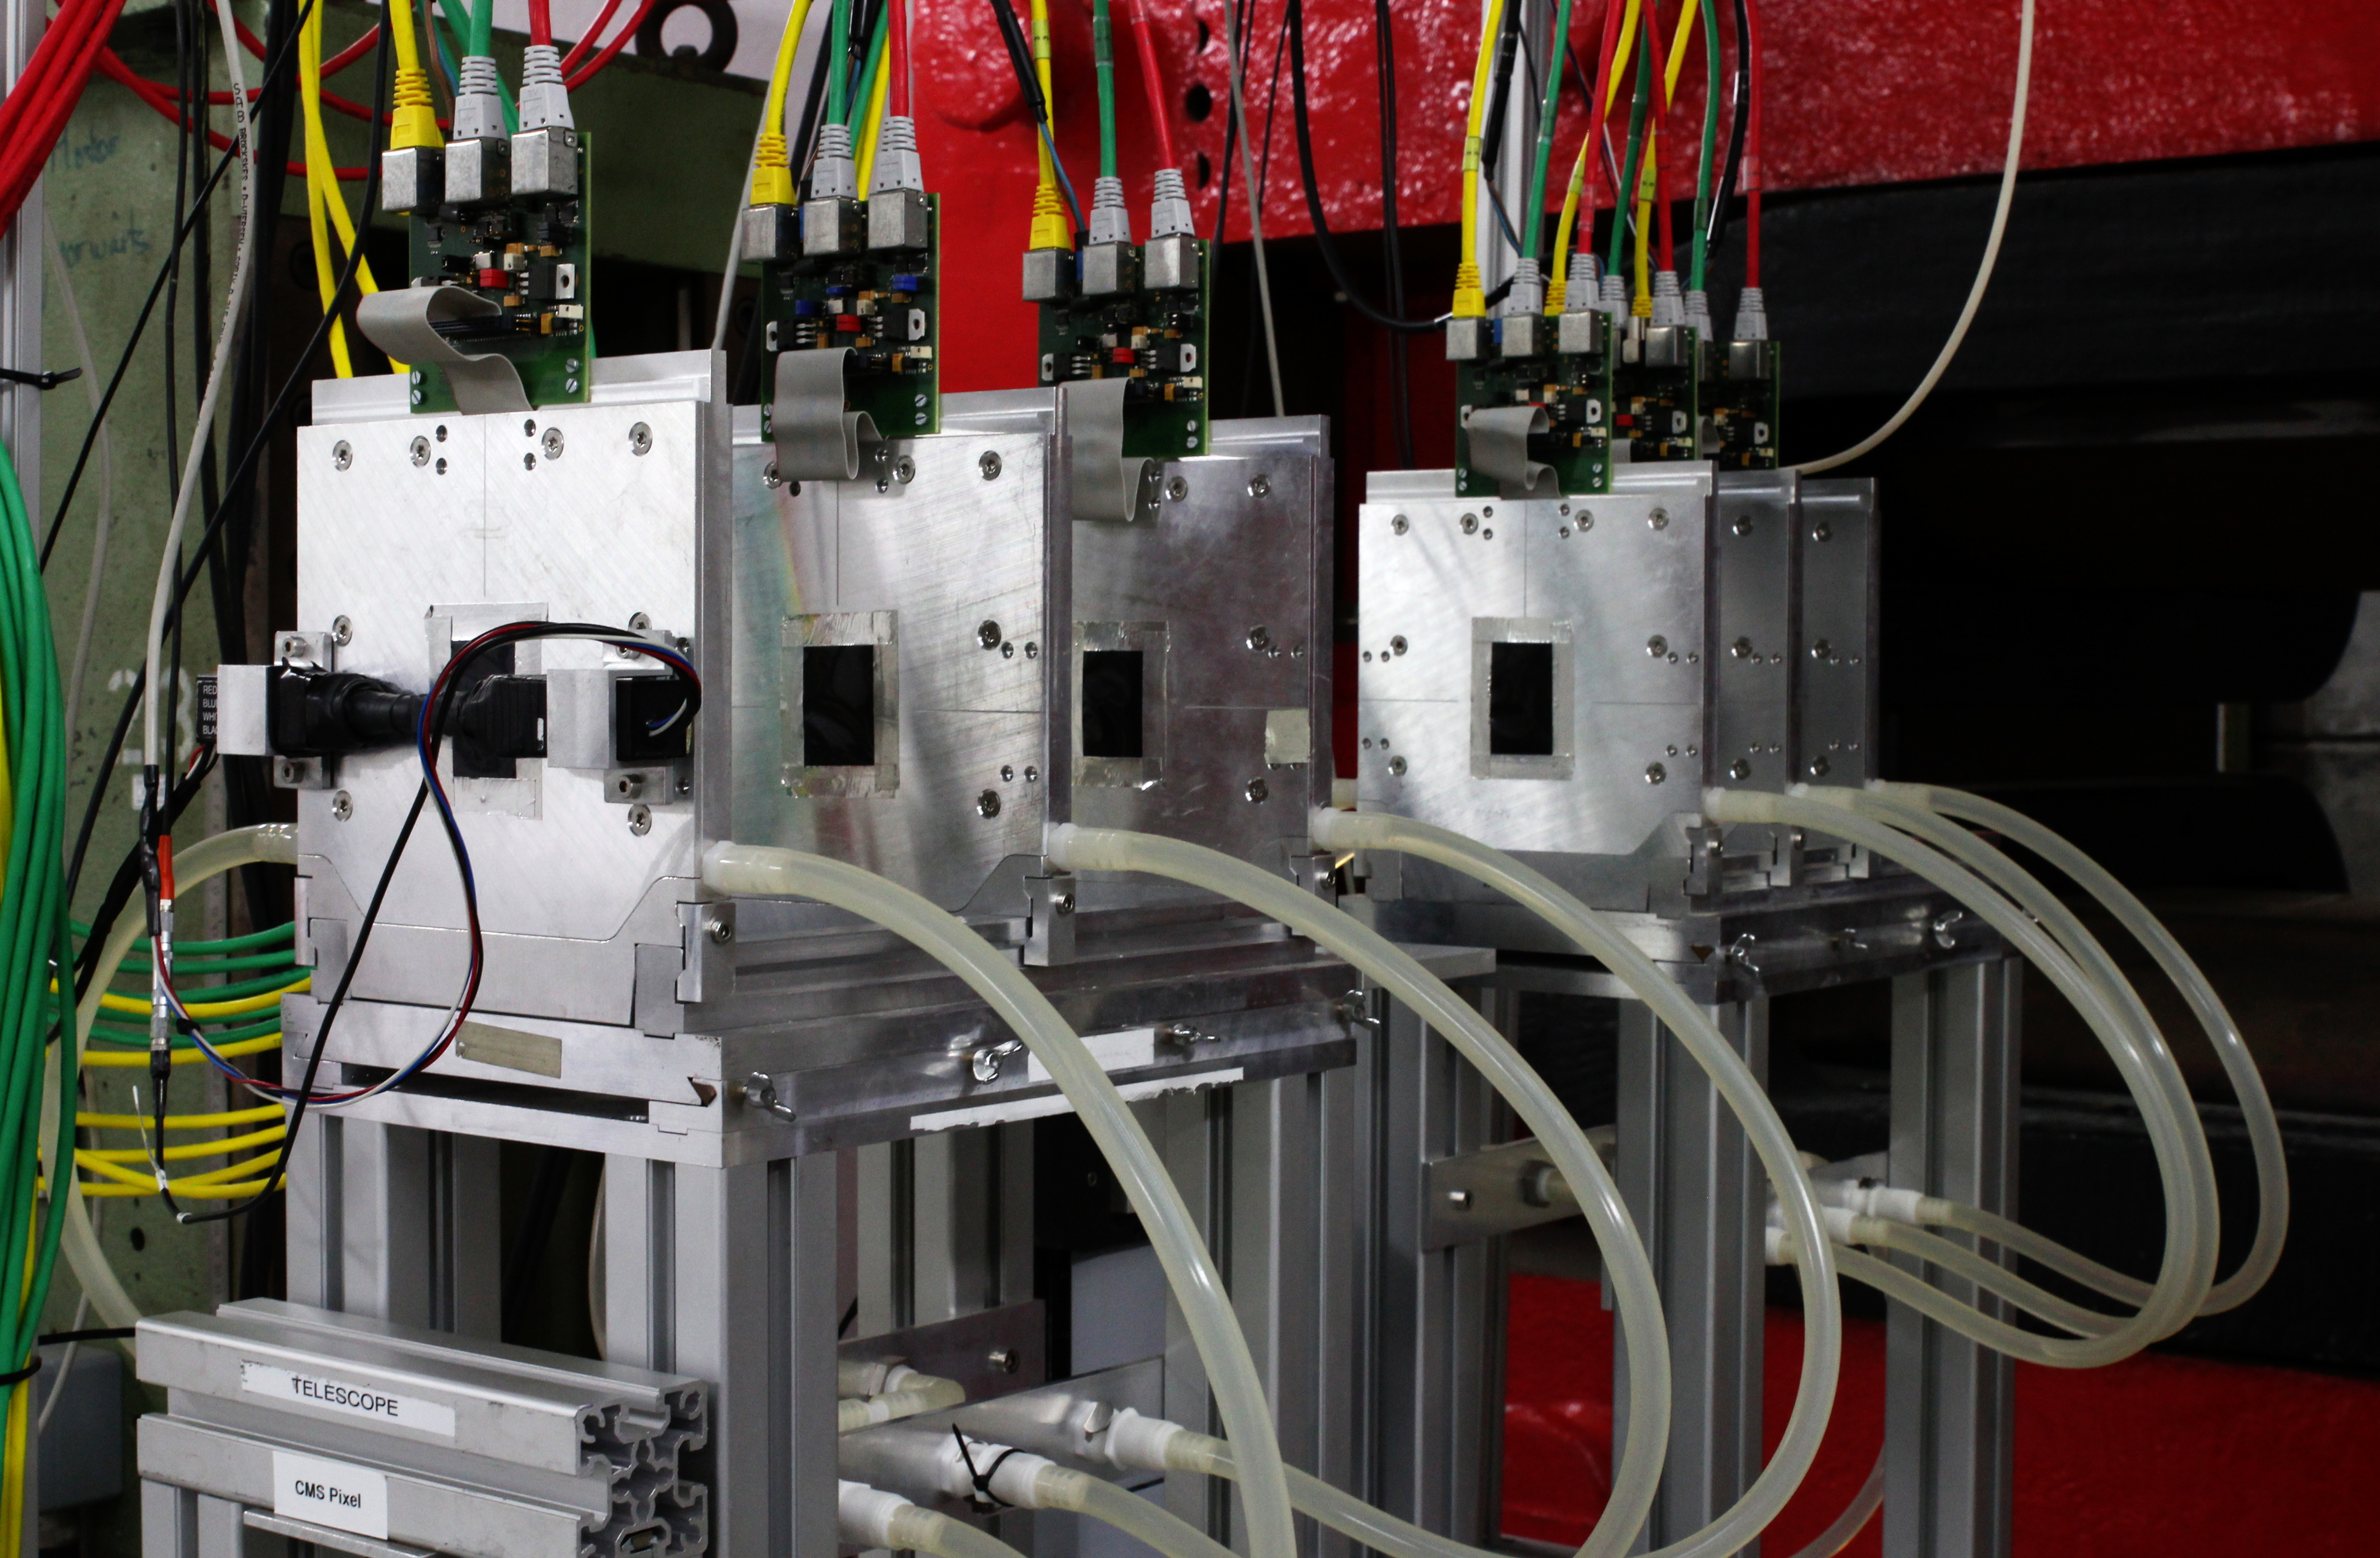
\includegraphics[width=.9\textwidth]{figures/DATURA.jpg}
	\caption[The $\Datura$ telescope]{The $\Datura$ beam telescope with its sensor planes on aluminium rails.
	The auxiliary boards with connections for clock signals, sensor configuration, and data lines are mounted at the top of the jigs.
	Coolant is provided to the jigs via the tubes.}
	\label{fig:datura-tscope}
\end{figure}
 
\subsection{Sensors and mechanics}

The $\Mimosa$ detectors used for precise spacial measurement of particle trajectories are manufactured with the 350\,nm CMOS technology. 
Each $\Mimosa$ detector consists of pixels sized $\unit{18.4}{\upmu\meter} \times \unit{18.4}{\upmu\meter}$, which are arranged in 1152 columns and 576 rows.\,\cite{HuGuo2010480}
This adds to a total of about four million readout channels covering an active area of about $\unit{10.6}{\milli\meter} \times \unit{21.1}{\milli\meter}$. 
The $\Mimosa$ sensors have been thinned down to $\unit{50}{\upmu\meter}$ and are protected on each side by $\unit{25}{\upmu\meter}$ lightproof Kapton foil. 
Free charge carriers produced in the underlying \unit{14}{\upmu\meter} epitaxial layer are mainly collected via diffusion. 
The binary resolution of $\unit{5.3}{\upmu\meter}$ can be improved by charge sharing, as will be shown in section~\ref{sec:trackres}.
%With the rising industrial interest in high resistivity epitaxial silicon for CMOS detectors the production cost of improved noise and radiation hardness parameters
% became already possible with ~400 Ohm·cm for 10 μm epitaxial layer for $\Mimosa$. 

The $\Mimosa$ sensors are read out with a rolling-shutter, taking 16\,cycles of an 80\,MHz clock per row, with all columns being read out in parallel. 
This allows for correlated double sampling and zero suppression on-chip with the digital circuitry placed outside the active pixel array. 
At this clock frequency, the $\Mimosa$ integration time equals $\unit{115.2}{\upmu\second}$ and allowing for about 8680 frames to be read out per second. 
The expected maximum rate of detectable particles through the active area estimates to be about $\unit{1}{\mega\hertz/\centi\meter^2}$ due to the limited on-chip buffer size. 
The detection threshold is programmable via so-called JTAG files. 
These provide configurations with different threshold levels in integer multiples of the RMS noise $\noise$ of the individual planes. 
A sensor threshold setting of six therefore corresponds to a collected charge in a single pixel of at least six times the noise. 
The average noise occupancy per read-out frame is measured to be smaller than $2\cdot10^{-5}$ at room temperature and a signal-to-noise threshold of six.

Every pixel sensor is mounted within an aluminium jig, three jigs are in turn mounted on each of the two aluminium arms. 
The jigs feature a beam window around the position of the sensor location, minimising the material budget. 
The overall material of the beam telescope thus amounts to $\unit{300}{\upmu\meter}$ of silicon and $\unit{300}{\upmu\meter}$ of Kapton. 
The two telescope arms, usually one up- and one downstream of the DUT, is movable along the direction of the beam in order to allow for variably sized DUTs to be fitted into the set-up. 
The minimal distance between two sensors is given by the jig thickness of 20\,mm, the maximal distance is restricted by the length of the aluminium arms to 150\,mm at equidistant spacing.
Furthermore, the jigs are cooled keeping the $\Mimosa$ sensors at a constant temperature allowing for stable operation.
The entire beam telescope is placed on a rotatable frame easing adjustment of its orientation parallel to the beam. 
Additionally, this frame is mounted on a sturdy structure providing stability over time and wheels for easy transportation. 

Important parameters are compiled in figure~\ref{fig:datura_sketch}. 
The distance between $\Mimosa$ planes is denoted as $\dz$, the distance between the DUT and its nearest neighbouring $\Mimosa$ planes $\dzdut$. 
The expression $\varepsilon = \sum_i x_{i}/X_{0,i}$ defines the material budget of the scattering medium as the material thickness normalised to its radiation lengths,
 with values of $X_0 = 93.65\,\milli\meter$ for silicon, $X_0 = 3.042\cdot 10^{5}\,\milli\meter$ for dry air, and $X_0 = 285.6\,\milli\meter$ for Kapton.\,\cite{ref:x0values}
The material budget of a $\Mimosa$ plane including a protecting Kapton foil on each side is $\epsmimo = 0.00071$. 
Likewise, the DUT's material budget is called $\epsdut$ and includes the DUT itself and other material such as PCBs and cooling boxes.


te edit: something about radiation lengths here...
\label{sec:radiationlengths}
with values of $X_0 = 21.82\,\allowbreak\gram\per\centi\meter^2$ for silicon and $X_0 = 36.62\,\gram\per\centi\meter^2$ for dry air, according to reference~\cite{ref:x0values}.


\begin{figure}[tb]
	\center
	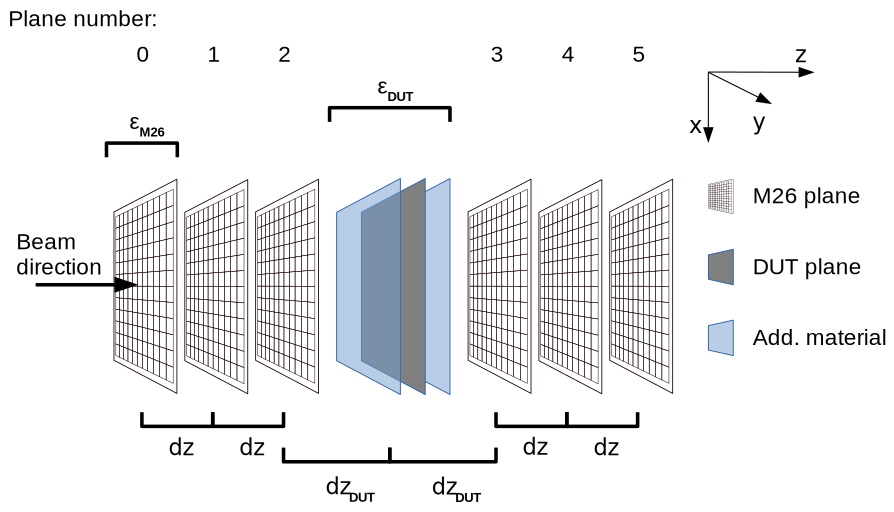
\includegraphics[width=.9\textwidth]{figures/sketch_tscope4}
	\caption[Sketch of the DESY-type telescope set-up]{Sketch of the DESY-type telescope set-up and its important parameters.}
	\label{fig:datura_sketch}
\end{figure}

\subsection{Trigger and DAQ system}

Four Hamamatsu PMTs assemblies with scintillators and lightguides, two in front and two in the back of the telescope, define the spatial acceptance window for triggers. 
The crossed scintillators on either side of the beam telescope define a rectangular acceptance window of $10\,\milli\meter \times 20\,\milli\meter$ matching the $\Mimosa$ acceptance area. 
The TLU, based on a commercial Spartan\,3 board, features a coincidence unit with discriminator boards accepting up to four PMT inputs signals. 
Additionally, it is equipped with several custom-made add-on PCBs allowing for an easy integration of user DAQ systems. 
Providing a programmable logic, the TLU  takes a trigger decision and distributes the trigger signal to all DAQ systems.
As interface to the beam telescope DAQ and other DUTs, the TLU provides RJ45 connectors with four LVDS pairs carrying the trigger clock, the busy line, the reset line, and a trigger line. 
The data clock and the busy line are inputs to the TLU, whereas the reset and the trigger line are outputs. 
Also a LEMO interface is available accepting busy, reset, and trigger. 
The TLU accepts a busy signal from each integrated device individually halting the issue of the next trigger if the busy signal is high. 
The handling of the trigger/busy signals can be done in three handshake modes, one being the ``no-handshake'' mode,
 in which the TLU issues a fixed-length pulse on the trigger line with the busy line being disregarded. 
In simple handshake mode, the assertion of a trigger is replied by the DUTs by asserting a signal on the busy line. 
The TLU then de-asserts the trigger, and waits for busy going low on the busy line in order to be able to issue a subsequent trigger.
The normal handshake uses the same scheme as in the simple trigger mode, but additionally trigger data is transferred on the trigger line:
After the trigger has been de-asserted, the trigger number is clocked out via this line using the rising edges of the trigger clock as clock enable for the shift register holding the trigger data. 
The reset line is used to signal the reset of the timestamp counter.

The $\Mimosa$ sensors provide zero-suppressed hit data over a flat ribbon cable to the auxiliary boards, which provide RJ45 connectors to connect them with the
 data concentrator board collecting the data from all six sensors and the trigger/busy lines from the TLU. 
A 52-pin cable then transports the data and the TLU trigger/busy lines in parallel into a FlexRIO board, which is equipped with analogue-to-digital converters and an FPGA. 
The $\Mimosa$ data from the rolling-shutter readout is written continuously to RAM without taking into account the trigger information. 
The data is then available via direct memory access to the DAQ software framework and an event is written to disk in normal handshake mode, only if a trigger has been raised for a certain telescope readout frame. 

\subsection{DUT integration}

DUTs are integrated the same way as the telescope itself using either the RJ45 or the LEMO interface. 
An $xy\upphi$-stage is available for translation over the acceptance region and rotation of the DUT. 
The maximum DUT size when placed between the telescope arms is 500\,mm ?!.
was noch ?


\section{EuDAQ}
\label{sec:eudaq}

The modular cross platform data acquisition framework \eudaq~\cite{ref:eudaqwebsite} has been designed and developed to serve as flexible and simple to use data taking software for the DESY-type telescopes,
 allowing easy integration of other devices. 
It consist of completely independent modules communicating via TCP/IP enabling a distributed data acquisition with modules running on separate machines. 
Currently, \eudaq\ is designed for synchronous DAQ systems requiring one event per trigger per attached subdetector system before building the global event. 
Thus, the trigger rate is always limited by the slowest device.

The central interaction point for users with the framework is the Run Control and its graphical user interface (GUI). 
All other modules connect to the Run Control at startup and receive additional information from there during operation such as the commands for starting and stopping a DAQ run. 
The GUI provides all controls necessary to the user on shift. 
Another important user interface is the Log Collector, gathering logging information from all modules displaying them in one unified logging window. 
Log files are stored with recorded data files for later reference.

The actual detector data is delivered to the framework by so-called Producers.
Producers are the links between the EUDAQ framework and the subdetector systems such as the telescope, the TLU, or the user DAQ system.
They interface with the EUDAQ library and provide a set of commands to be called by the Run Control. 
This simple interface scheme eases the integration of user DAQ systems into the software framework.
The data read out from the detectors by the individual producers is sent to the so-called Data Collector. 
This Data Collector is repsonsible for the event building, i.e.\ the correlation of events from all subdetector systems to single global events comprising all data belonging to one trigger. 
Basic sanity checks such as the event numbers from the individual subdetectors are executed.

To ensure data quality during data acquisition the Online Monitor tool is avaliabe. 
It connects to the Data Collector requesting a fixed fraction of the recorded events (e.g.\ one out of a hundered) to fully decode all subdetector data
 and build basic plots such as hit maps or correlation plots showing that the different devices are synchronized in time and are all within the geometrical trigger acceptance.

The data decoding is done using Data Converter plugins for every detector type attached to the Run Control. 
The plugin to be called for a specific sub event can be deducted from the event type transmitted by the producer and written to the data stream by the Data Collector. 
Each Data Converter plugin can implement several data format end points to allow e.g.\ the conversion to an internal EUDAQ format for the Online Monitor, to simple ROOT trees, or to LCIO
 which is used by the offline reconstruction software described in the following section.

Configuration of the data acquisition framework is performed via global configuration files. 
The information for every individual module is parsed and distributed by the Run Control. 
The configuration file is a plain text file divided into sections for the individual modules, which contain a list of parameter-value pairs defined by the module.
The full content of the configuration file including commented lines is stored in the so-called Begin-Of-Run Event (BORE) of every run and is thus available later for offline analysis and reference. 
This greatly simplifies book keeping of detector parameters during test beam shifts since all settings are stored automatically.


\section{Offline analysis and reconstruction using EUTelescope}
\label{sec:offline}


For offline analysis and reconstruction of telescope test beam data the EUTelescope software package~\cite{ref:eudetmemo_2010_12,ref:eutelwebsite}
 is available and features a close integration of the EUDAQ software framework described in section~\ref{sec:eudaq}.
EUTelescope is based on the ILCSoft framework~\cite{ref:eudetmemo_2009_12} which provides the basic building blocks for offline analysis such as a generic data model (Linear Collider I/O, LCIO),
a geometry description language (GEAR) and the central event processor (Marlin) \cite{ref:eudetreport_2007_11}.

%\cite{EUDET-2008-48}.
Marlin allows for a modular composition of analysis chains for various applications. Every task is implemented as an independent processor which is called by Marlin for every event. 
Each processor exposes a set of parameters to the user which can be configured and loaded at runtime via so-called steering files in XML format.
This way the Marlin/Processor architecture gives maximum flexibility to the user.

\begin{figure}[tbp]
  \center
  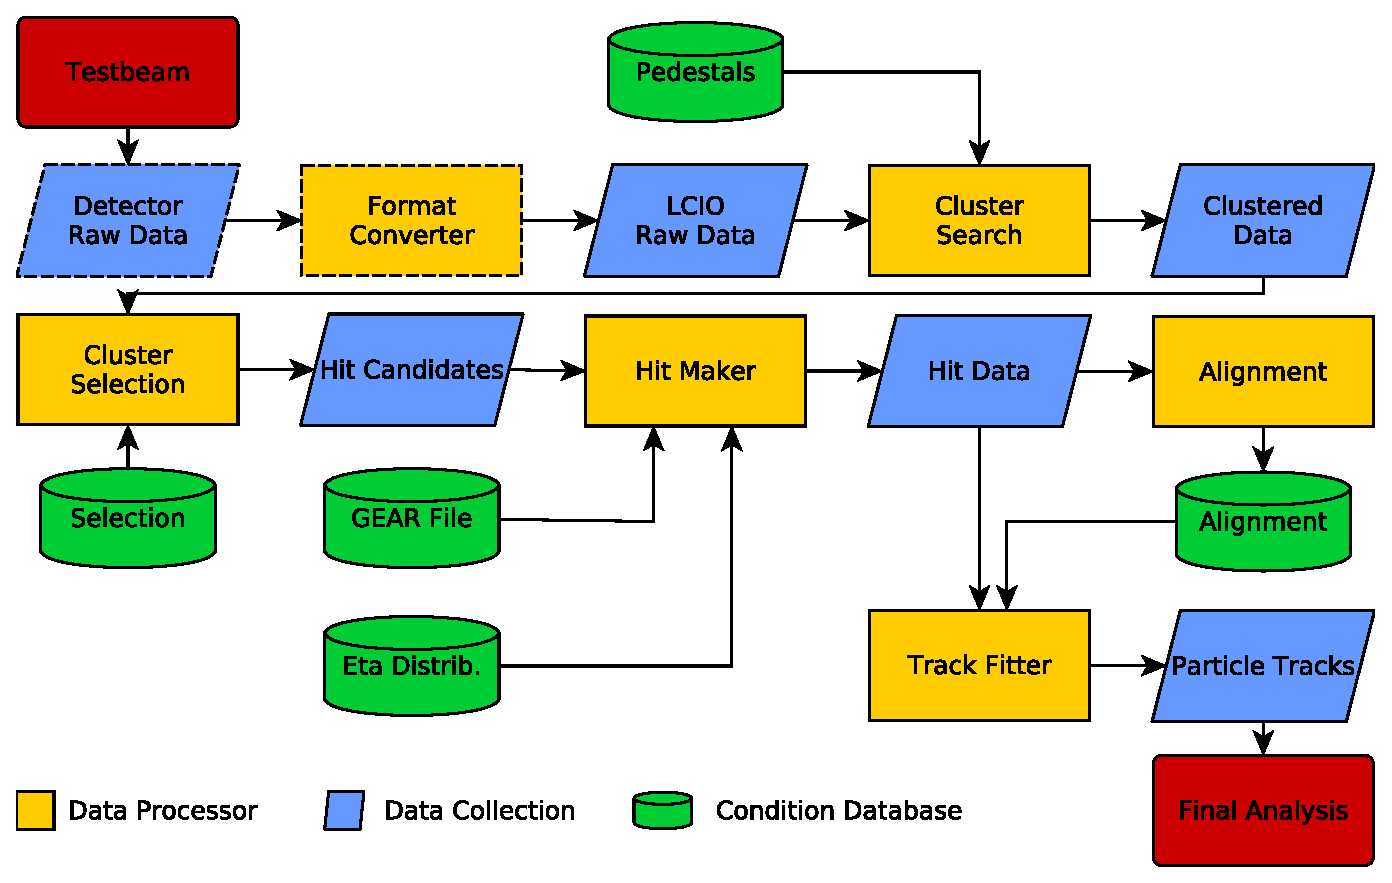
\includegraphics[width=.9\textwidth]{figures/eutel-strategy}
  \caption[The EUTelescope data analysis strategy]{Schematic of the overall telescope data reconstruction and analysis strategy of the EUTelescope framework.
EUTelescope provides processors for all steps, except for the conversion of the DUT raw data, marked with a dashed outline.}
  \label{fig:offline:strategy}
\end{figure}

EUTelescope provides several processors for Marlin, implementing algorithms necessary for a full track reconstruction and data analysis of test beam experiments. 
Figure~\ref{fig:offline:strategy} shows the analysis strategy of the framework starting from the recorded detector response to the final reconstructed particle tracks. 
%An overview of the processor range provided by EUTelescope is given in \cite{EUDET-2007-20}.
At low-energy beam lines such as the DESY-II test beam facility, multiple scattering is an important contribution to the overall track resolution uncertainty,
 especially in measurements with non-negligible DUT material budget, cf.\ section~\ref{sec:multiplescattering}.
Therefore, EUTelescope provides processors implementing advanced algorithms for tracking such as Deterministic Annealing Filter (DAF)~\cite{ref:daffitter}
 or GBL which account for scattering in all material present in the beam.
For high-energy beam lines a simple straight line fit provides sufficient precision and a maximum of computational performance.
In addition, precise offline detector alignment can be performed by minimising track residuals using the EUTelescope alignment processor which utilises the Millepede-II algorithm~\cite{Blobel-2006}.

EUTelescope comes with its own job submission framework Jobsub that allows to run analysis jobs on local machines or to submit them to larger computing clusters such as NAF for bulk reconstruction.
Using its flexible configuration file concept and the global run database storing user defined variables,
 jobsub eases the implementation of per-run variables for reconstruction such as beam energy or detector alignment.

 
The track parameters are calculated by employing a $\chi^{2}$-minimisation method~\cite{ref:eudetmemo_2007_01,ref:lutzpaper}.
For each telescope sensor dimension ($x$ and $y$), the individual contribution $\Delta \chi^2_{i}$ from plane $i$ is defined as

\begin{equation}
\label{eq:chi2contrib}
\Delta \chi^2_{i} = \left( \frac{r - p_{i}}{\sigmai} \right)^2 \Bigg|_{i \ne i_{\textrm{DUT}}} +
\left( \frac{\theta_{\textrm{i}} - \theta_{i-1}}{\Theta_{0}} \right)^2 \Bigg|_{i \ne 0,N-1} \,,
\end{equation}

\noindent
with the telescope plane numbering beginning at zero.
The measured hit position in one dimension is denoted by $r$, the position extrapolated from the track in the same dimension by $p_{i}$.
The angles between the nominal beam direction and the track direction are $\theta_{i-1}$ and $\theta_{i}$.
The former is the track angle entering plane $i$, the latter the angle of the outbound track segment.
The intrinsic resolution of sensor plane $i$ and the width of the multiple scattering distribution are denoted $\sigmai$ and $\Theta_{0}$, respectively, cf.~also section~\ref{sec:multiplescattering}. 
It is assumed that $\sigmai$ and $\Theta_{0}$ do not differ between planes and that $\sigmai$ is also equal for both measurement dimensions.
If the beam axis is denoted by $z$, then $\theta_i$ can be expressed as

\begin{equation}
\theta_i = \frac{p_{i+1} - p_i}{z_{i+1} - z_i} \,.
\end{equation}

\noindent In equation~(\ref{eq:chi2contrib}) the first term, resulting from the hit measurement, is excluded in the $\chi^2$ calculation if the considered plane is the DUT.
Similarly, for the first and last planes the second term in equation~(\ref{eq:chi2contrib}) is omitted, since the scattering angle can not be determined.
This results in the global $\chi^2$ expression

\begin{equation}
\label{eq:globalchi2}
\chi^2 = \sum_{i=0}^{N-1} \alpha_i \left( r - p_i \right)^2 + \sum_{i=1}^{N-2}
\left( \frac{p_{i + 1} \beta_i + p_{i-1} \beta_{i-1} - p_i \left( \beta_i + \beta_{i-1} \right)}{\Theta_0} \right)^2 \,,
\end{equation}

\noindent
with coefficients $\alpha_i$ and $\beta_i$ defined as~\cite{ref:eudetmemo_2007_01}

\begin{equation}
\alpha_i = \left\{
  \begin{array}{l l}
    \sigmai^{-2} & \quad \text{for $i \neq i_{\textrm{DUT}}$}\\
    0 & \quad \text{for $i = i_{\textrm{DUT}}$}
  \end{array} \right. \quad \text{and} \quad \beta_i = \frac{1}{z_{i + 1} - z_i} \,.
\end{equation}

\noindent
which is minimised with respect to the track parameters $p_i$. 


\section{Track resolution}
\label{sec:trackres}

The telescope performance has been validated at CERN (120\,GeV pions) and DESY (1 to 6\,GeV positrons). 
In order to get realistic data description at DESY beam energies all scattering material between sensitive planes has to be taken into account. 
The precision of the track prediction at the DUT (plane \#3) based on five other telescope planes is shown in Figure\,\ref{fig:resolution}. 
The combination of the thickness of the telescope planes ($\unit{50}{\upmu\meter}$) with their hit position precision ($\sim\unit{3.5}{\upmu\meter}$)
 when minimising the distances to the Detector Under Test (DUT), 
 allows to sustain track pointing precision below $\unit{3}{\upmu\meter}$ for all electron (positron) energies above 2\,GeV and distance to the DUT shorter then 20\,mm (Figure\,\ref{fig:resolution}).


Fullquote~\cite{ref:thomas}
\bigskip


\section{Telescope Performance}\label{sec:telescoperesolution}

To verify the performance of the {DATURA} telescope, measurements of the
achievable resolution were performed in $2012$, for different settings of beam
momentum, sensor threshold and sensor spacing. With the \texttt{datura-noDUT}
example included in the {EUTelescope} framework, which is described in detail in
section~\ref{sec:datura-nodut}, straight line tracks with hits in all six
telescope planes were sought. From these tracks, the unbiased residual
distribution of each sensor plane was calculated. To calculate this
distribution, each of the six telescope planes was iteratively considered as a
DUT. Within each iteration, tracks were calculated from the five non-DUT planes.
The unbiased residual distribution was then filled by the distance between the
hit position and the track extrapolation in the DUT plane. By using each
telescope plane as a DUT, equation~\ref{eq:telescoperesolutionequation} is
modified under the assumption that $\sigma_{\textrm{Intrinsic}} =
\sigma_{\textrm{DUT}} = \sigma_{\textrm{M26}}$, leading to

\begin{equation}
\label{eq:telescoperesolutionequation_2}
\sigma_{\textrm{meas}}^2 = \sigma_{\textrm{M26}}^2 \cdot \left( 1 + k \right) +
\sigma_{\textrm{MS}}^2\,.
\end{equation}


Figure~\ref{fig:residualexample1} shows an example of residual distributions for
a telescope sensor spacing of $20\,\milli\meter$, a beam momentum of
$5\,\giga\electronvolt$ and a sensor threshold setting of $6$. The residual
distributions for the outer planes $0$ and $5$ are wider than the distributions
obtained from the inner sensors. This is due to the fact that the track
extrapolation to the inner sensors is done from both sides, hence will be
comparatively more precise than for the outer sensors, where the extrapolation
can only be performed from one direction. In all cases, the distributions are
fitted with a Gaussian, from which the residual width $\sigma_{\textrm{meas}}$
is determined.\\

\begin{figure}[hbtp]
\centering
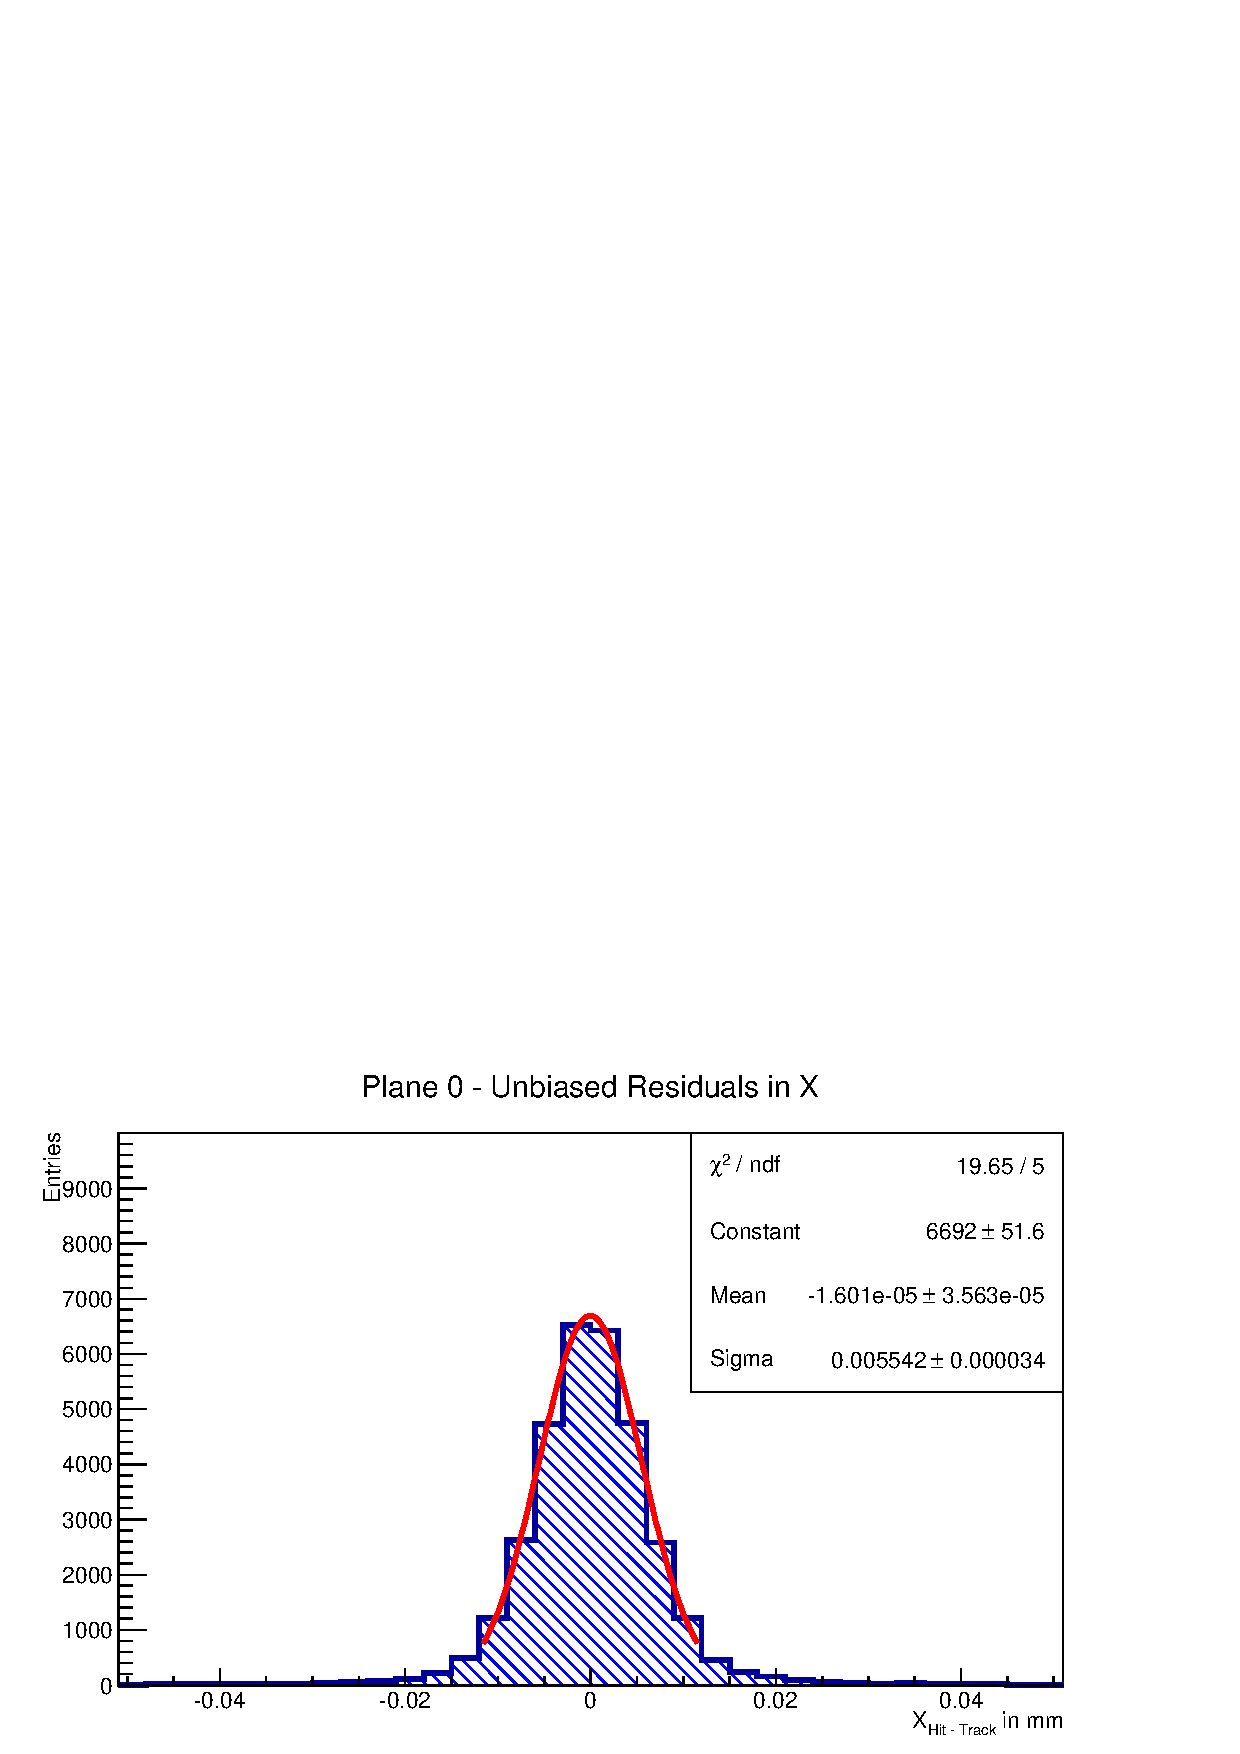
\includegraphics[width=0.45\textwidth]{gfk/chapter03/resis_upstream/0x.pdf}
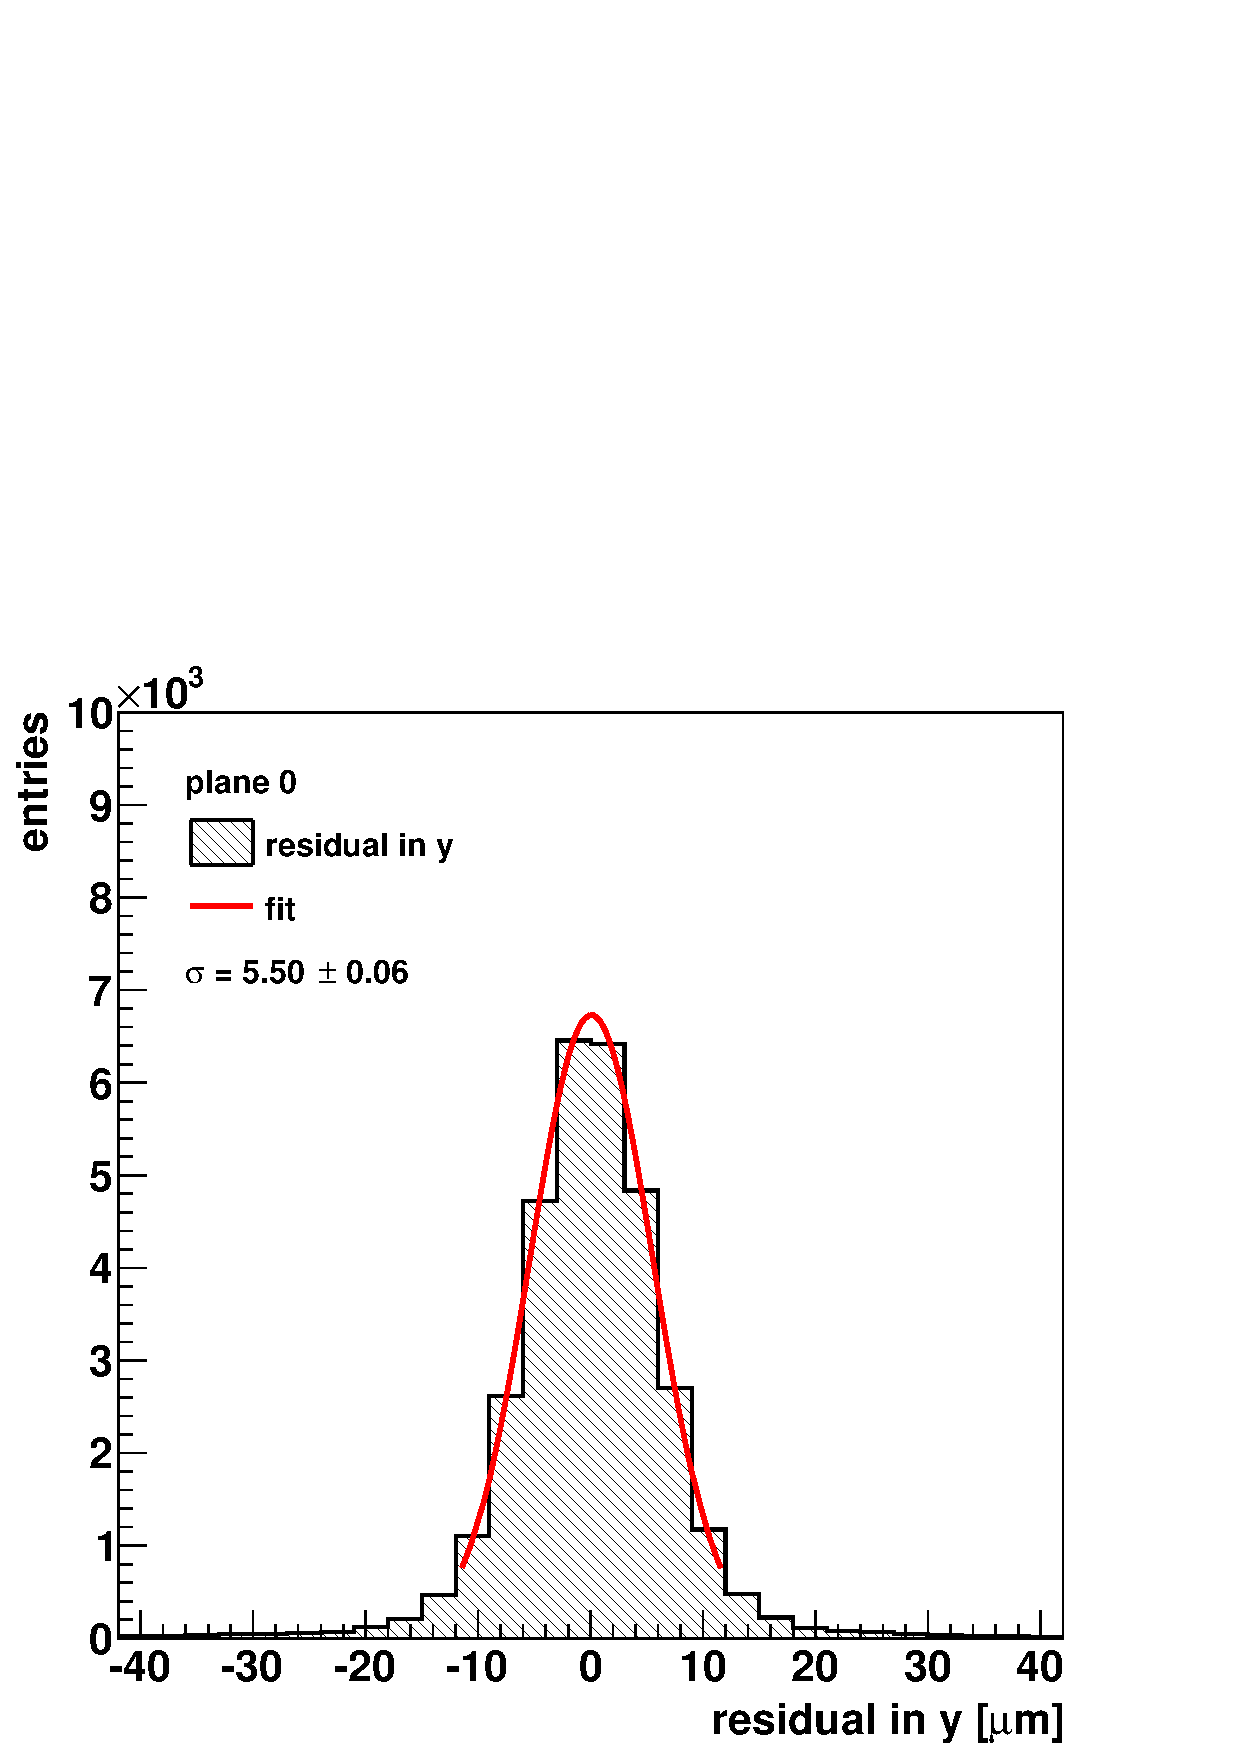
\includegraphics[width=0.45\textwidth]{gfk/chapter03/resis_upstream/0y.pdf}
\includegraphics[width=0.45\textwidth]{gfk/chapter03/resis_upstream/1x.pdf}
\includegraphics[width=0.45\textwidth]{gfk/chapter03/resis_upstream/1y.pdf}
\includegraphics[width=0.45\textwidth]{gfk/chapter03/resis_upstream/2x.pdf}
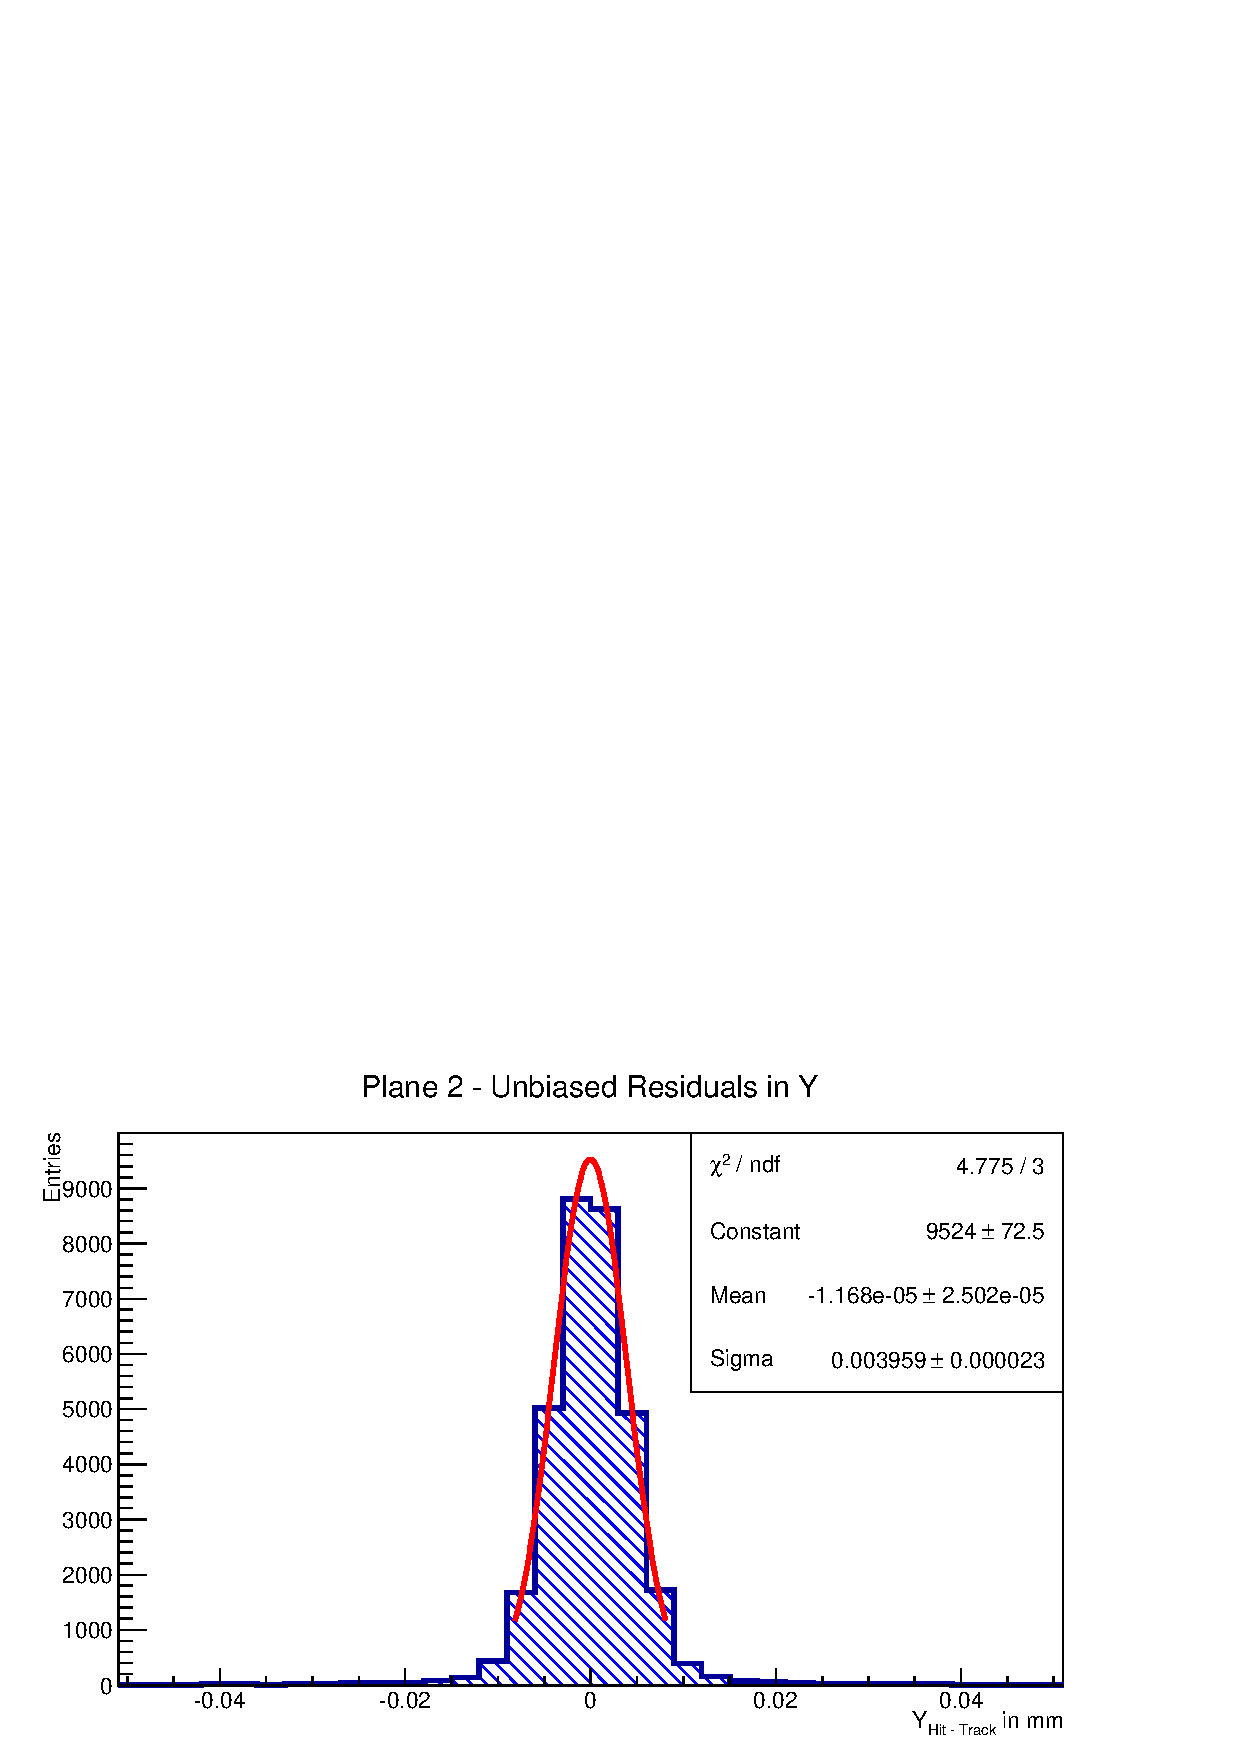
\includegraphics[width=0.45\textwidth]{gfk/chapter03/resis_upstream/2y.pdf}
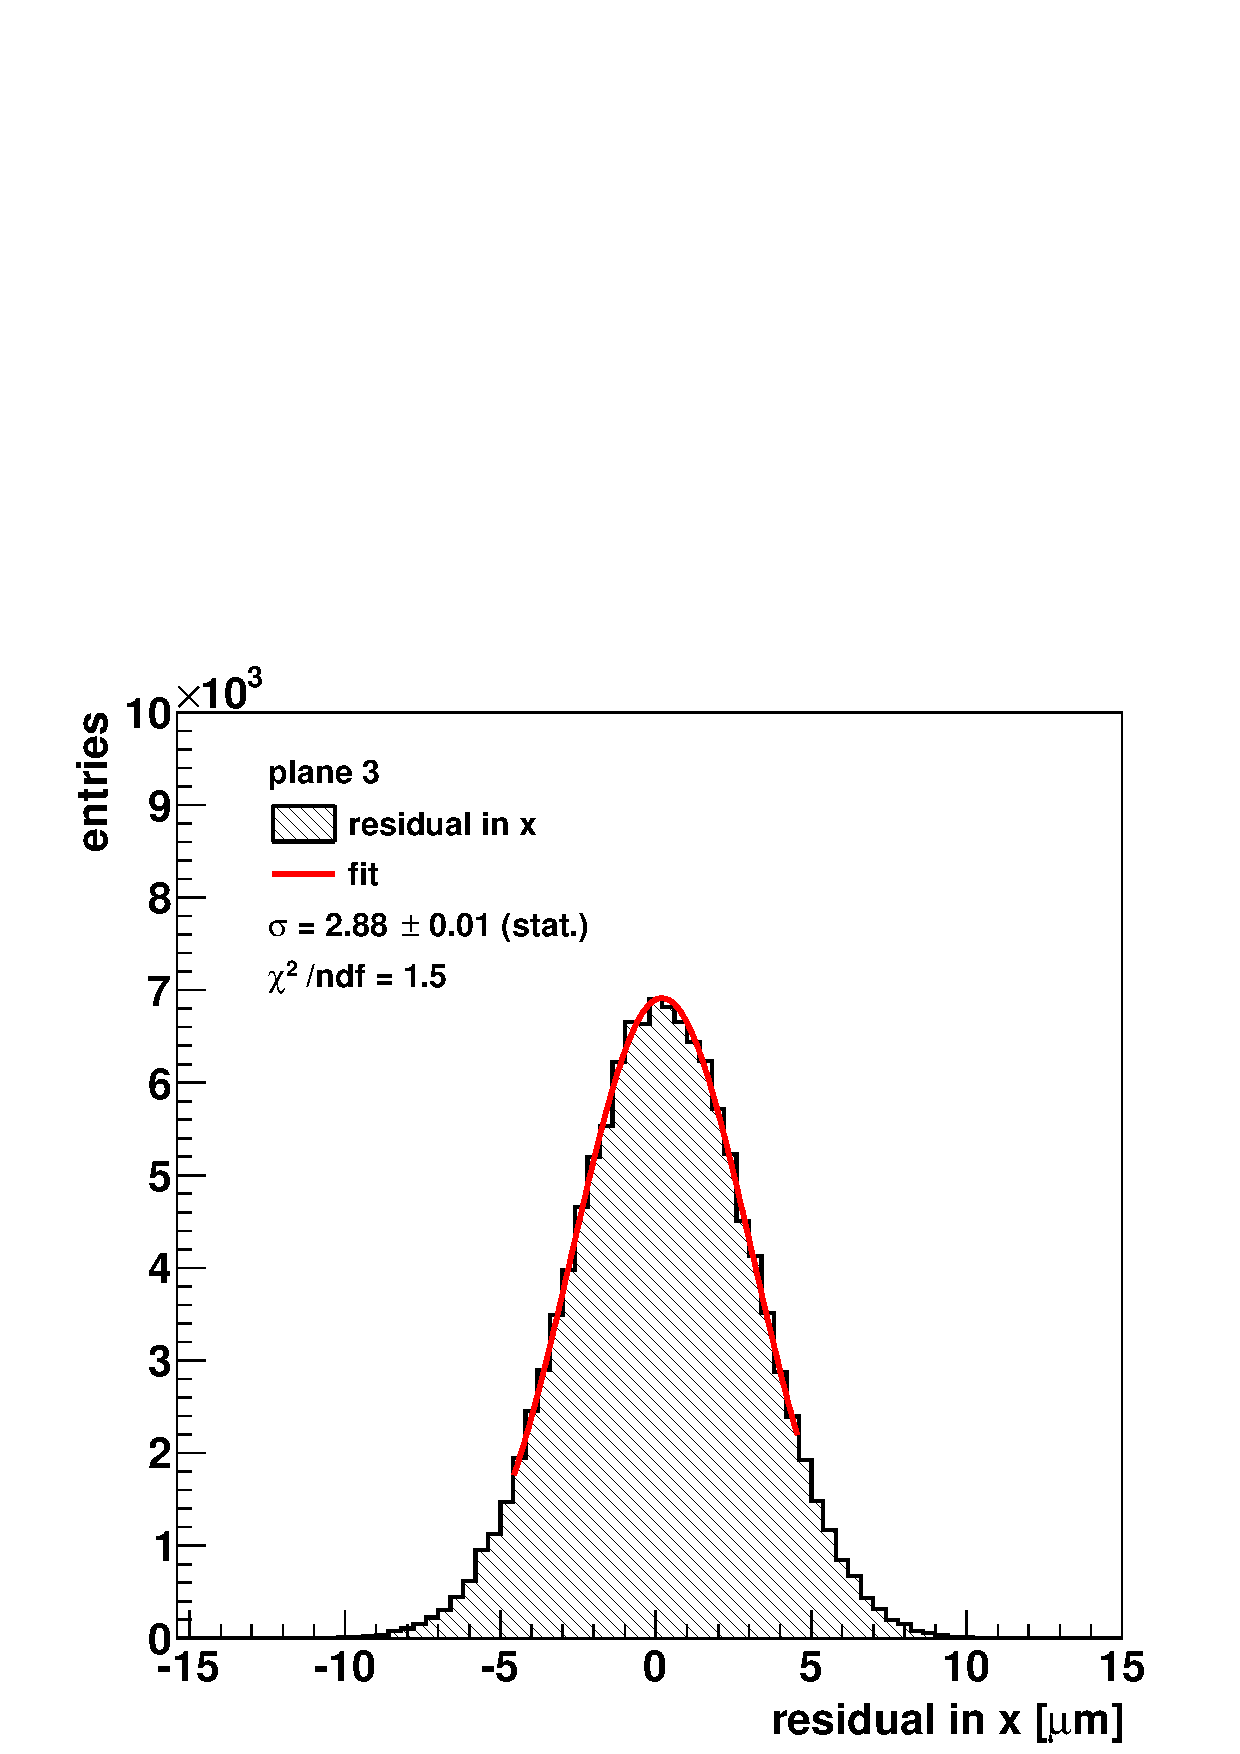
\includegraphics[width=0.45\textwidth]{gfk/chapter03/resis_downstream/3x.pdf}
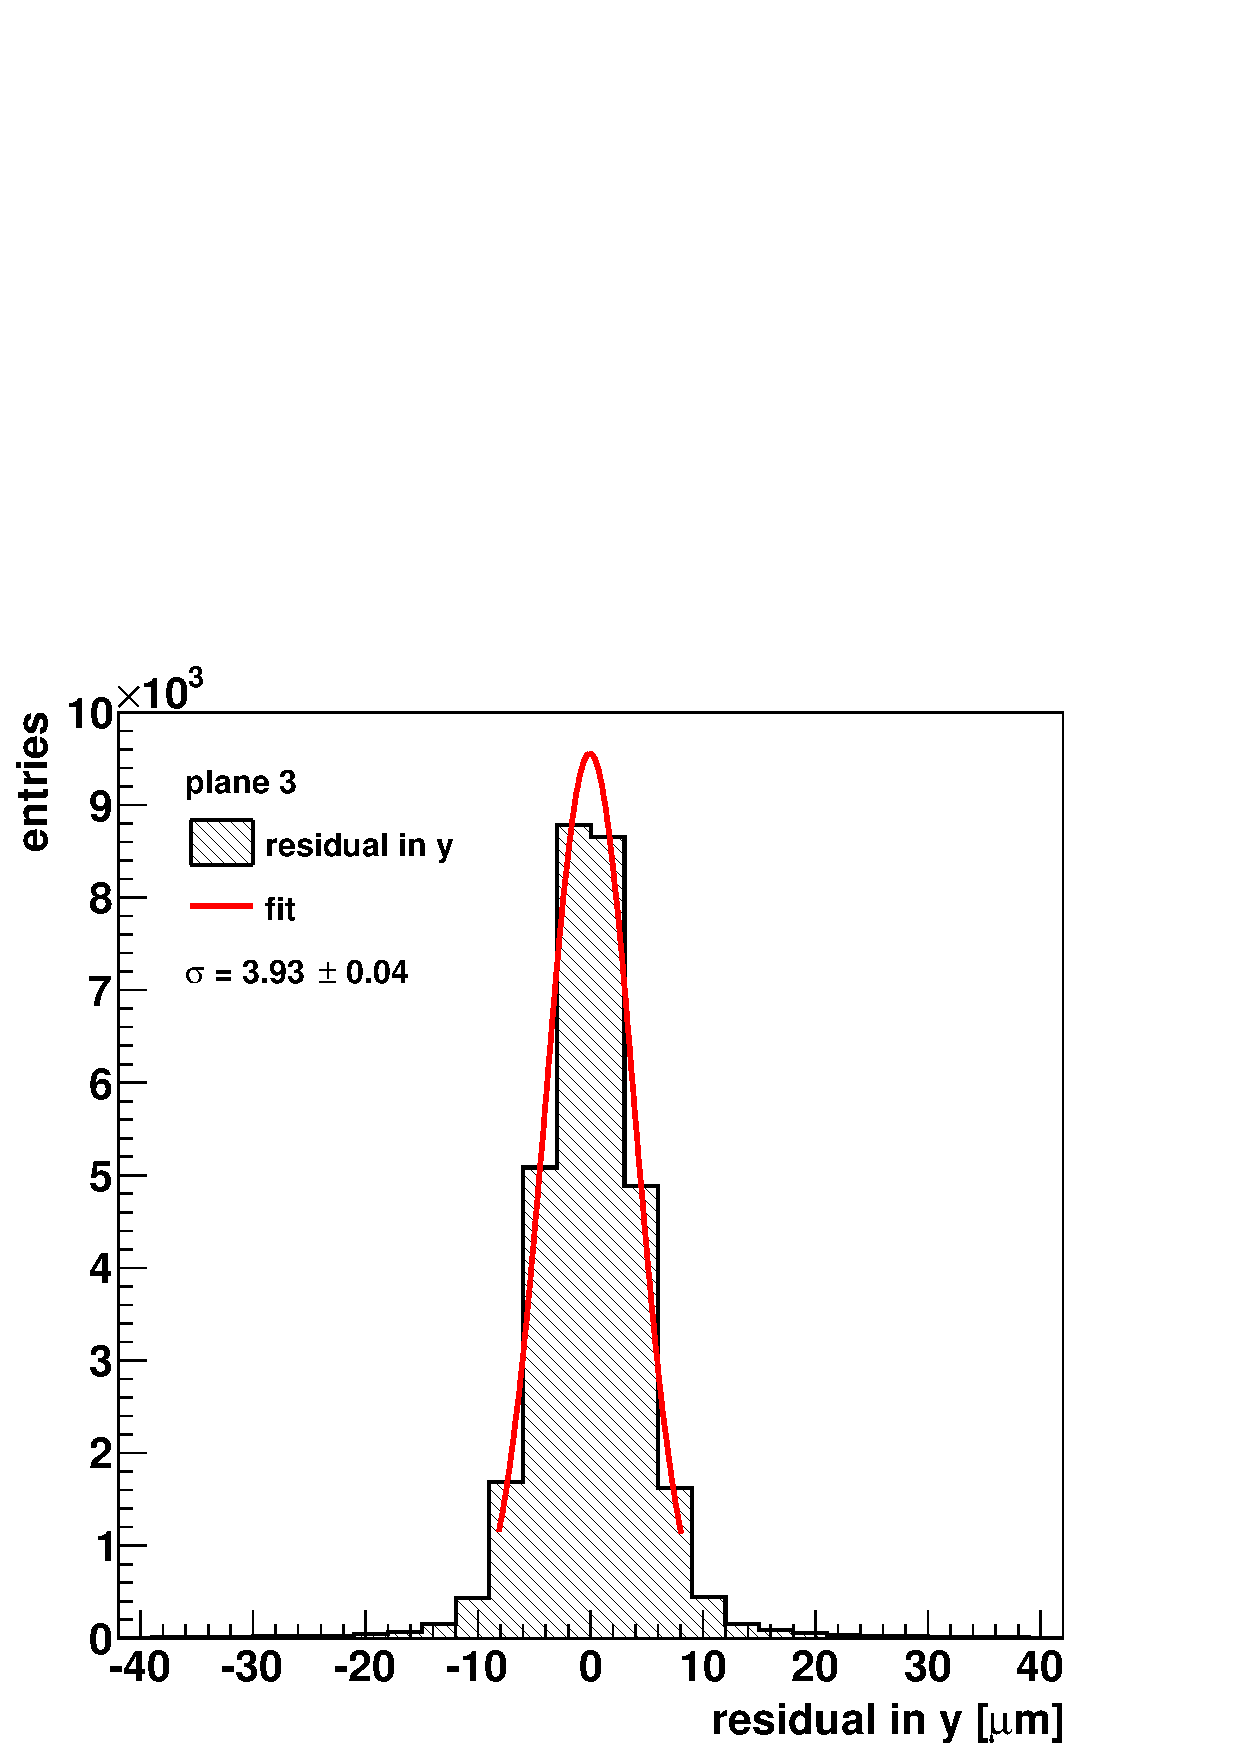
\includegraphics[width=0.45\textwidth]{gfk/chapter03/resis_downstream/3y.pdf}
\includegraphics[width=0.45\textwidth]{gfk/chapter03/resis_downstream/4x.pdf}
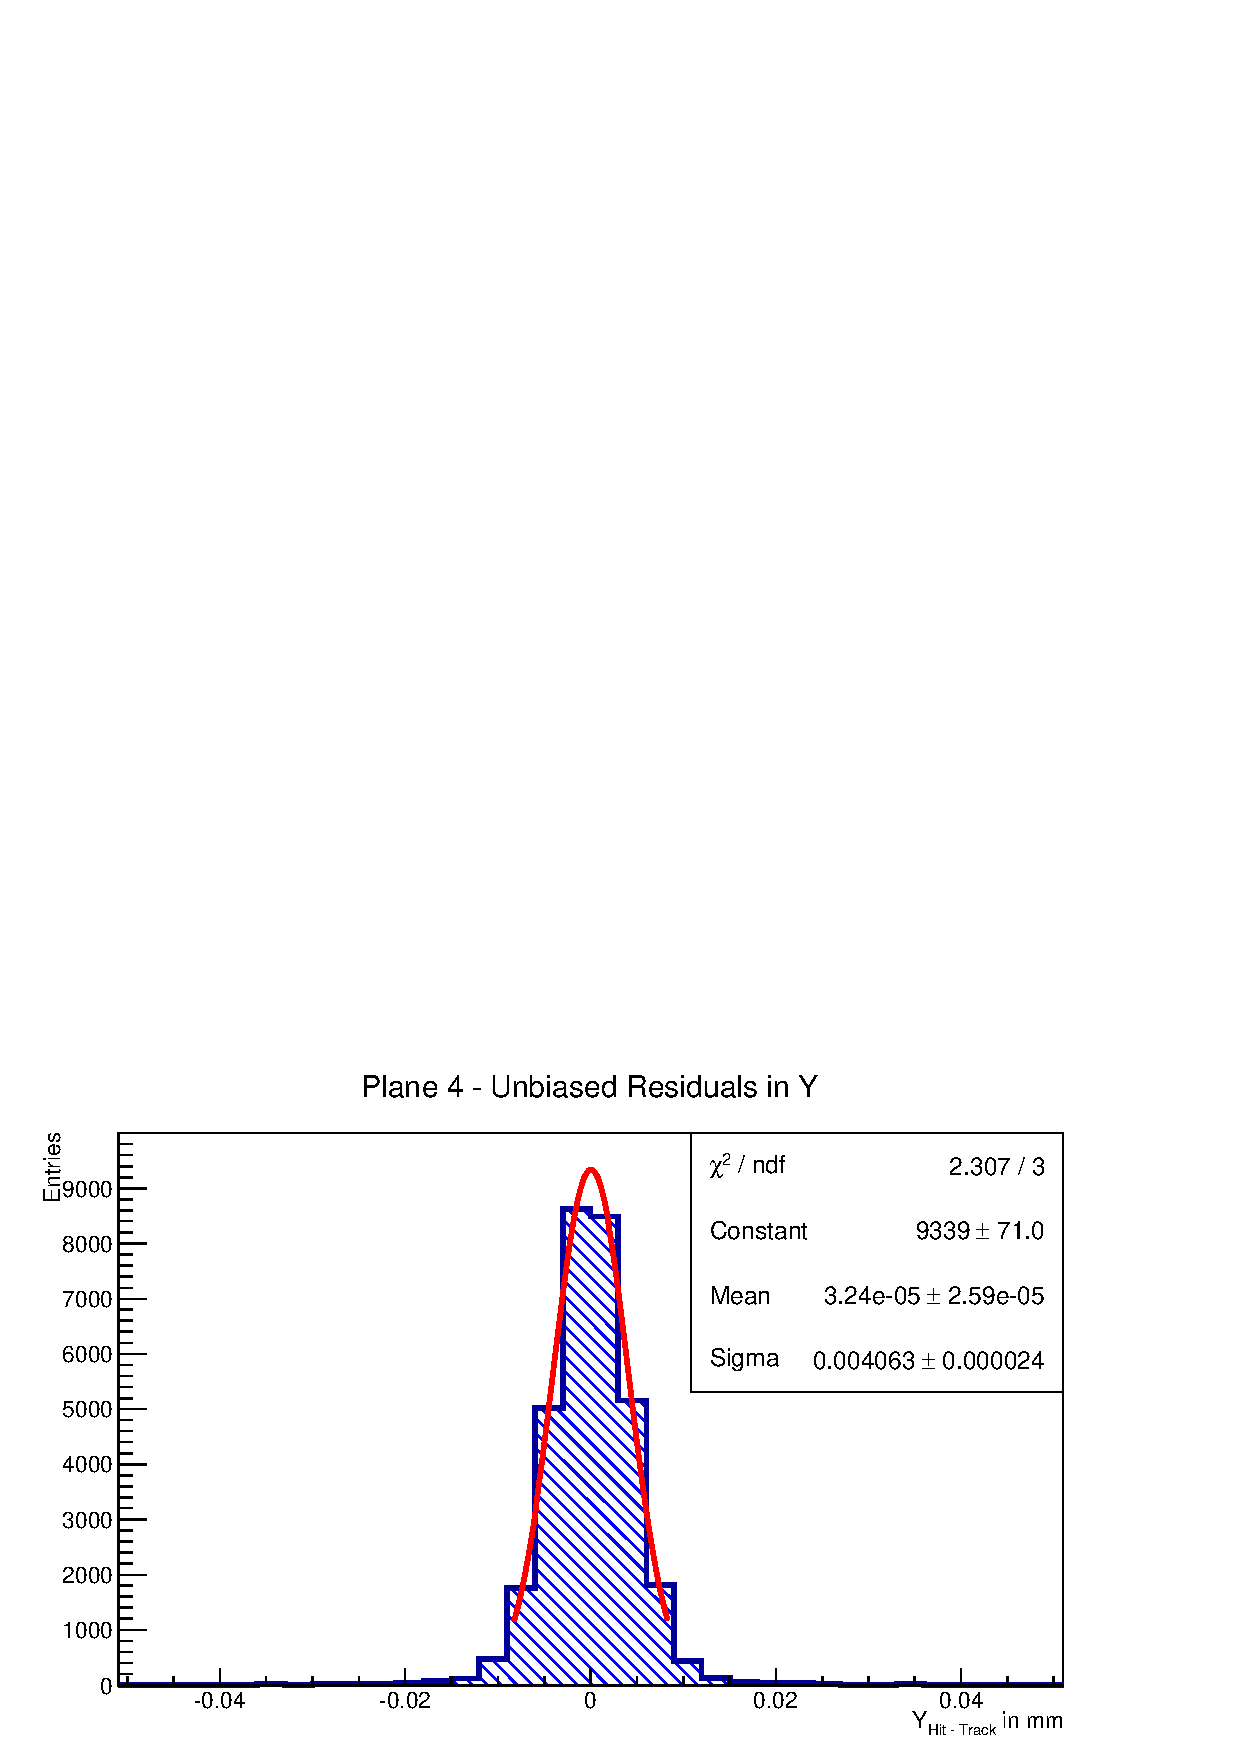
\includegraphics[width=0.45\textwidth]{gfk/chapter03/resis_downstream/4y.pdf}
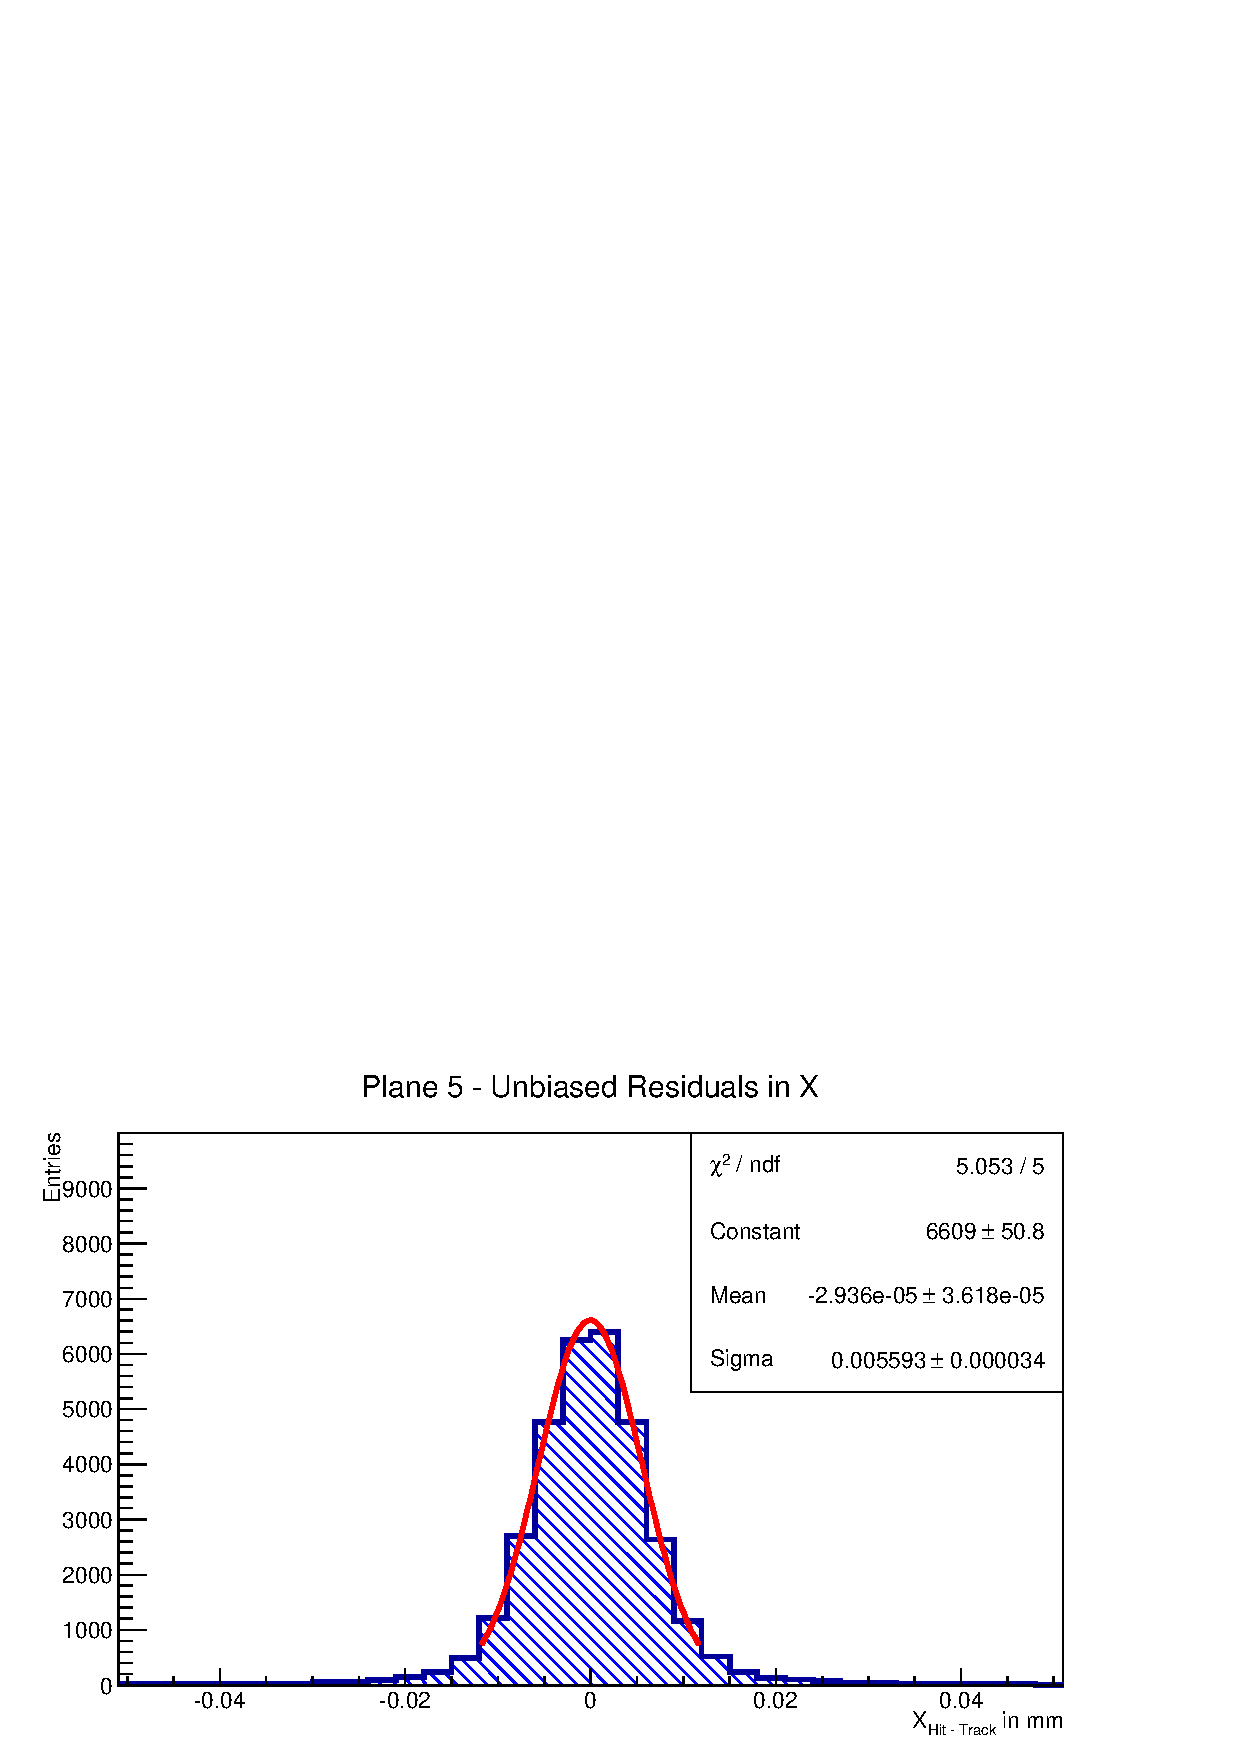
\includegraphics[width=0.45\textwidth]{gfk/chapter03/resis_downstream/5x.pdf}
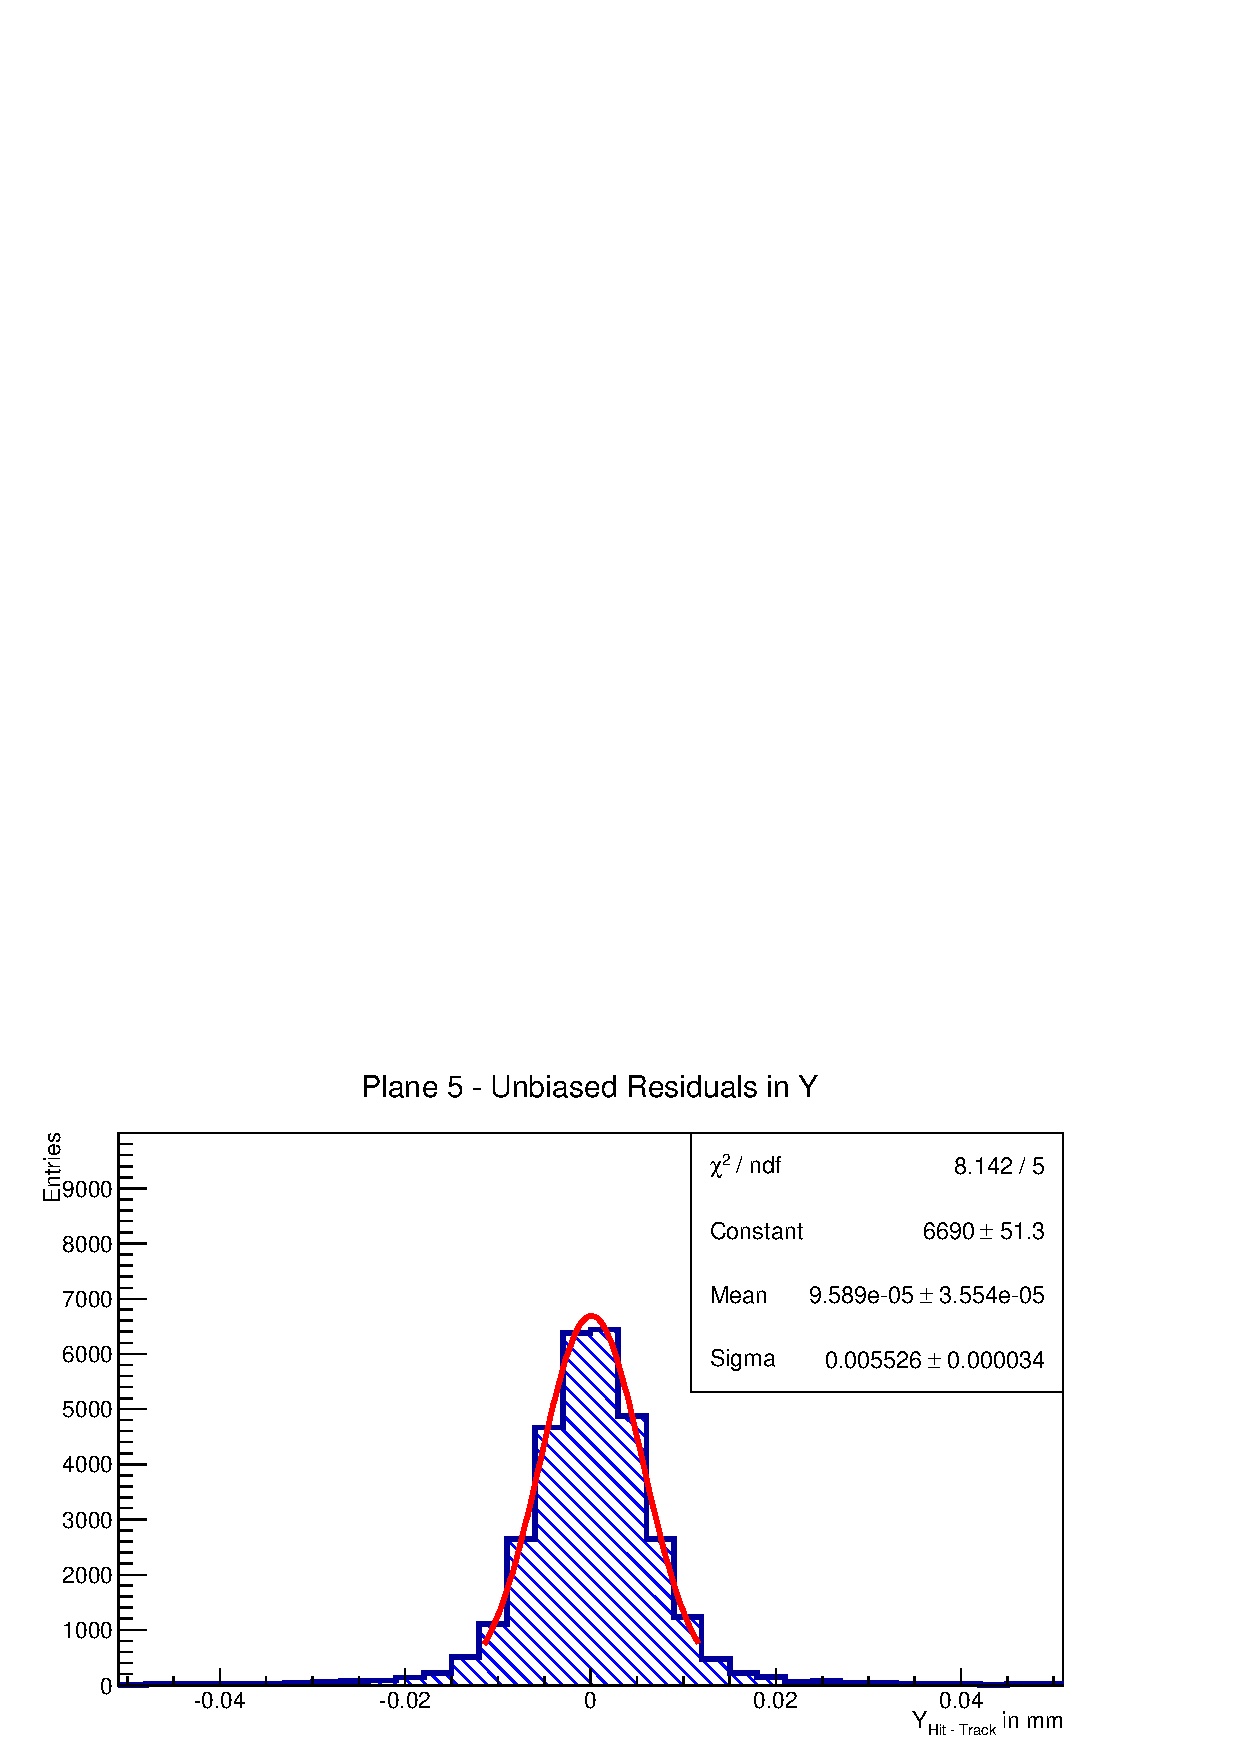
\includegraphics[width=0.45\textwidth]{gfk/chapter03/resis_downstream/5y.pdf}
\caption[Residual examples to determine the DATURA telescope's
resolution. Upstream lever arm]{Residual examples to determine the DATURA
telescope's resolution from the upstream lever arm. From top to bottom: The
measured residuals for planes $0$, $1$, $2$, $3$, $4$ and $5$, left for $X$
direction, right for $Y$ direction. Each sensor plane was considered as a
passive layer during the track reconstruction.}
\label{fig:residualexample1}
\end{figure}

\begin{comment}

\begin{figure}[hbtp]
\centering


\caption[Residual examples to determine the DATURA telescope's
resolution. Downstream lever arm]{Residual examples to determine the DATURA
telescope's resolution from the downstream lever arm. From top to bottom: The
measured residuals for planes $3$, $4$ and $5$, left for $X$ direction, right
for $Y$ direction. Each sensor plane was considered as a passive layer during
the track reconstruction.}
\label{fig:residualexample2}
\end{figure}

\end{comment}

By using a $\chi^{2}$ minimization method, the intrinsic resolution of the
{MIMOSA 26} telescope sensors was calculated from
equation~\ref{eq:telescoperesolutionequation_2}. The results for both a tighter
plane spacing of $20\,\milli\meter$ and a wider spacing of $150\,\milli\meter$
are shown in figures~\ref{fig:smileythin} and~\ref{fig:smileythick},
respectively.\\

\begin{figure}[hbtp]
\centering
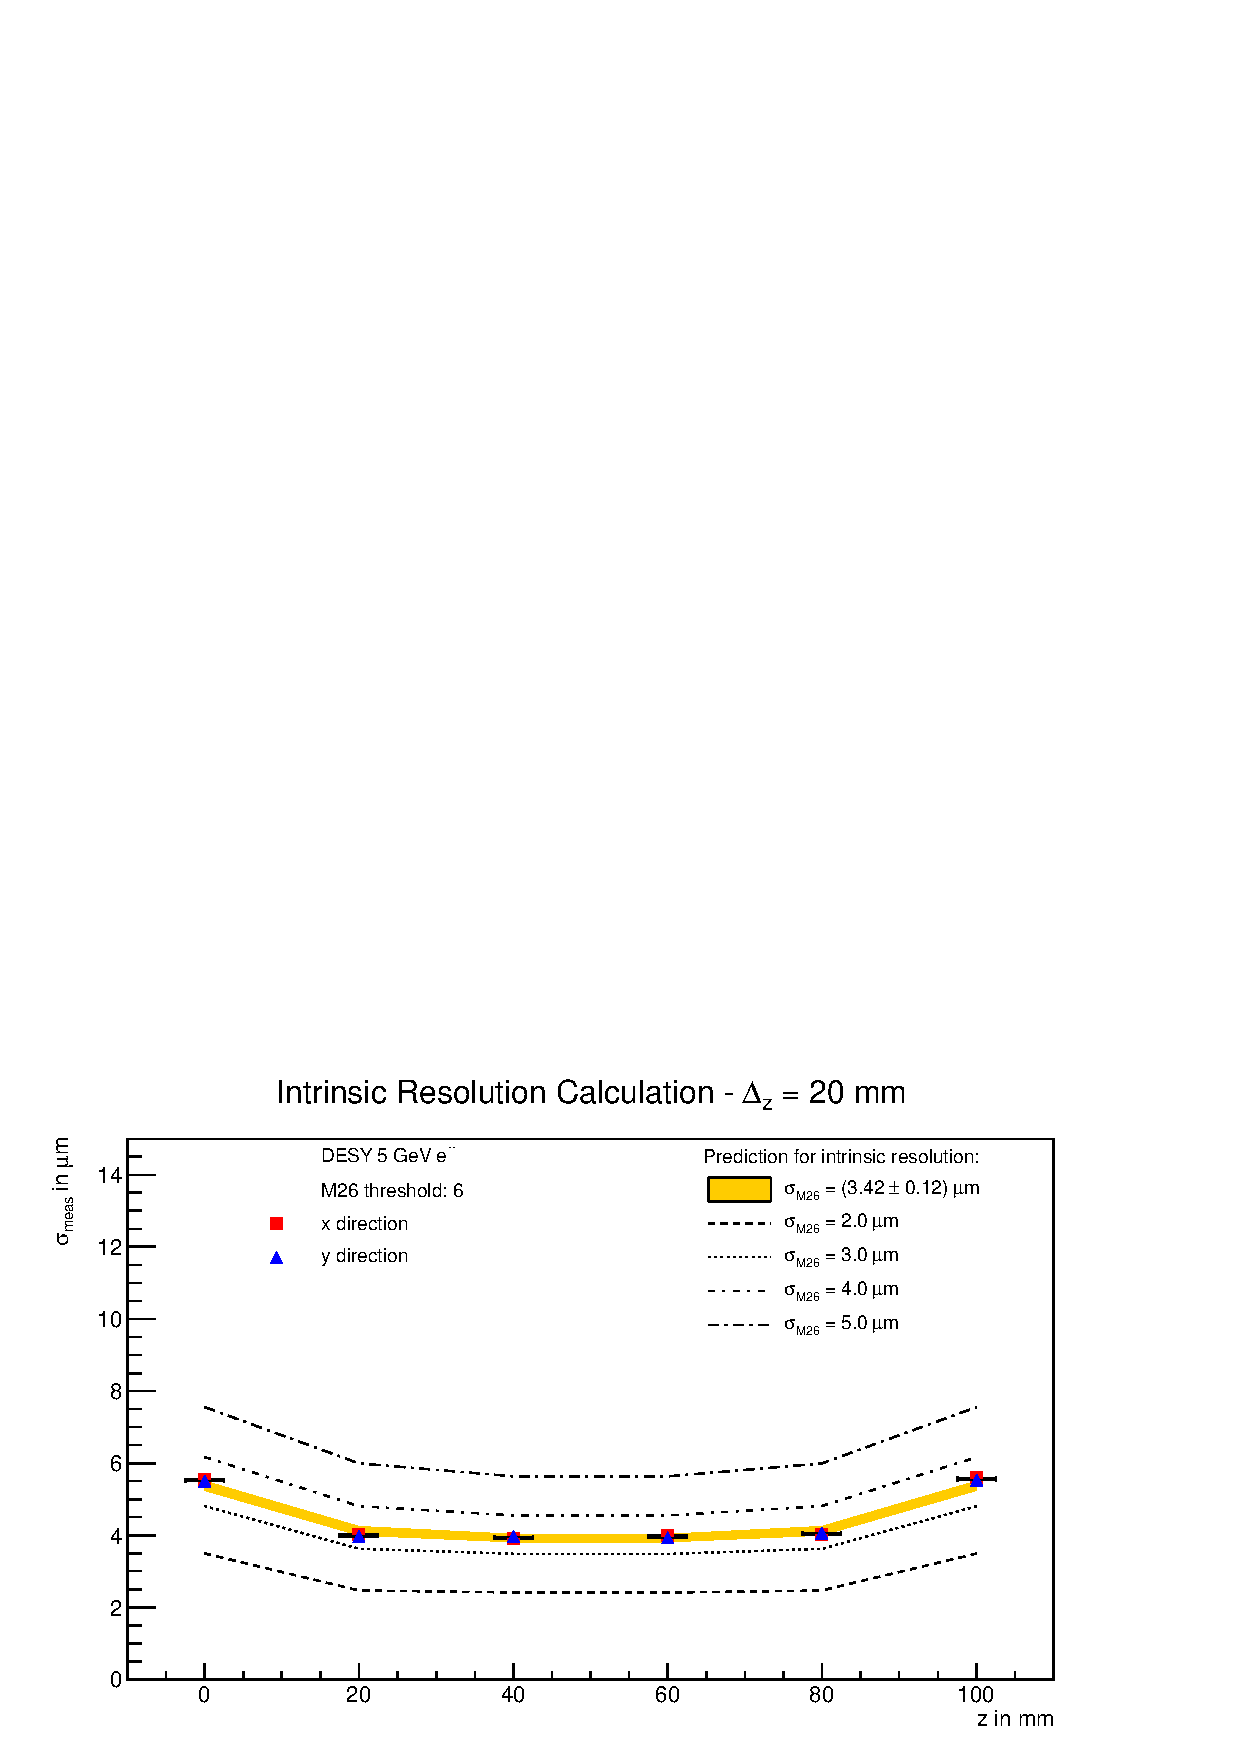
\includegraphics[width=\textwidth]{gfk/chapter03/thin_smiley.pdf}
\caption[Intrinsic telescope sensor resolution at $20\,\milli\meter$ plane
spacing]{Intrinsic telescope sensor resolution at $20\,\milli\meter$ plane
spacing.}
\label{fig:smileythin}
\end{figure}



\begin{figure}[hbtp]
\centering
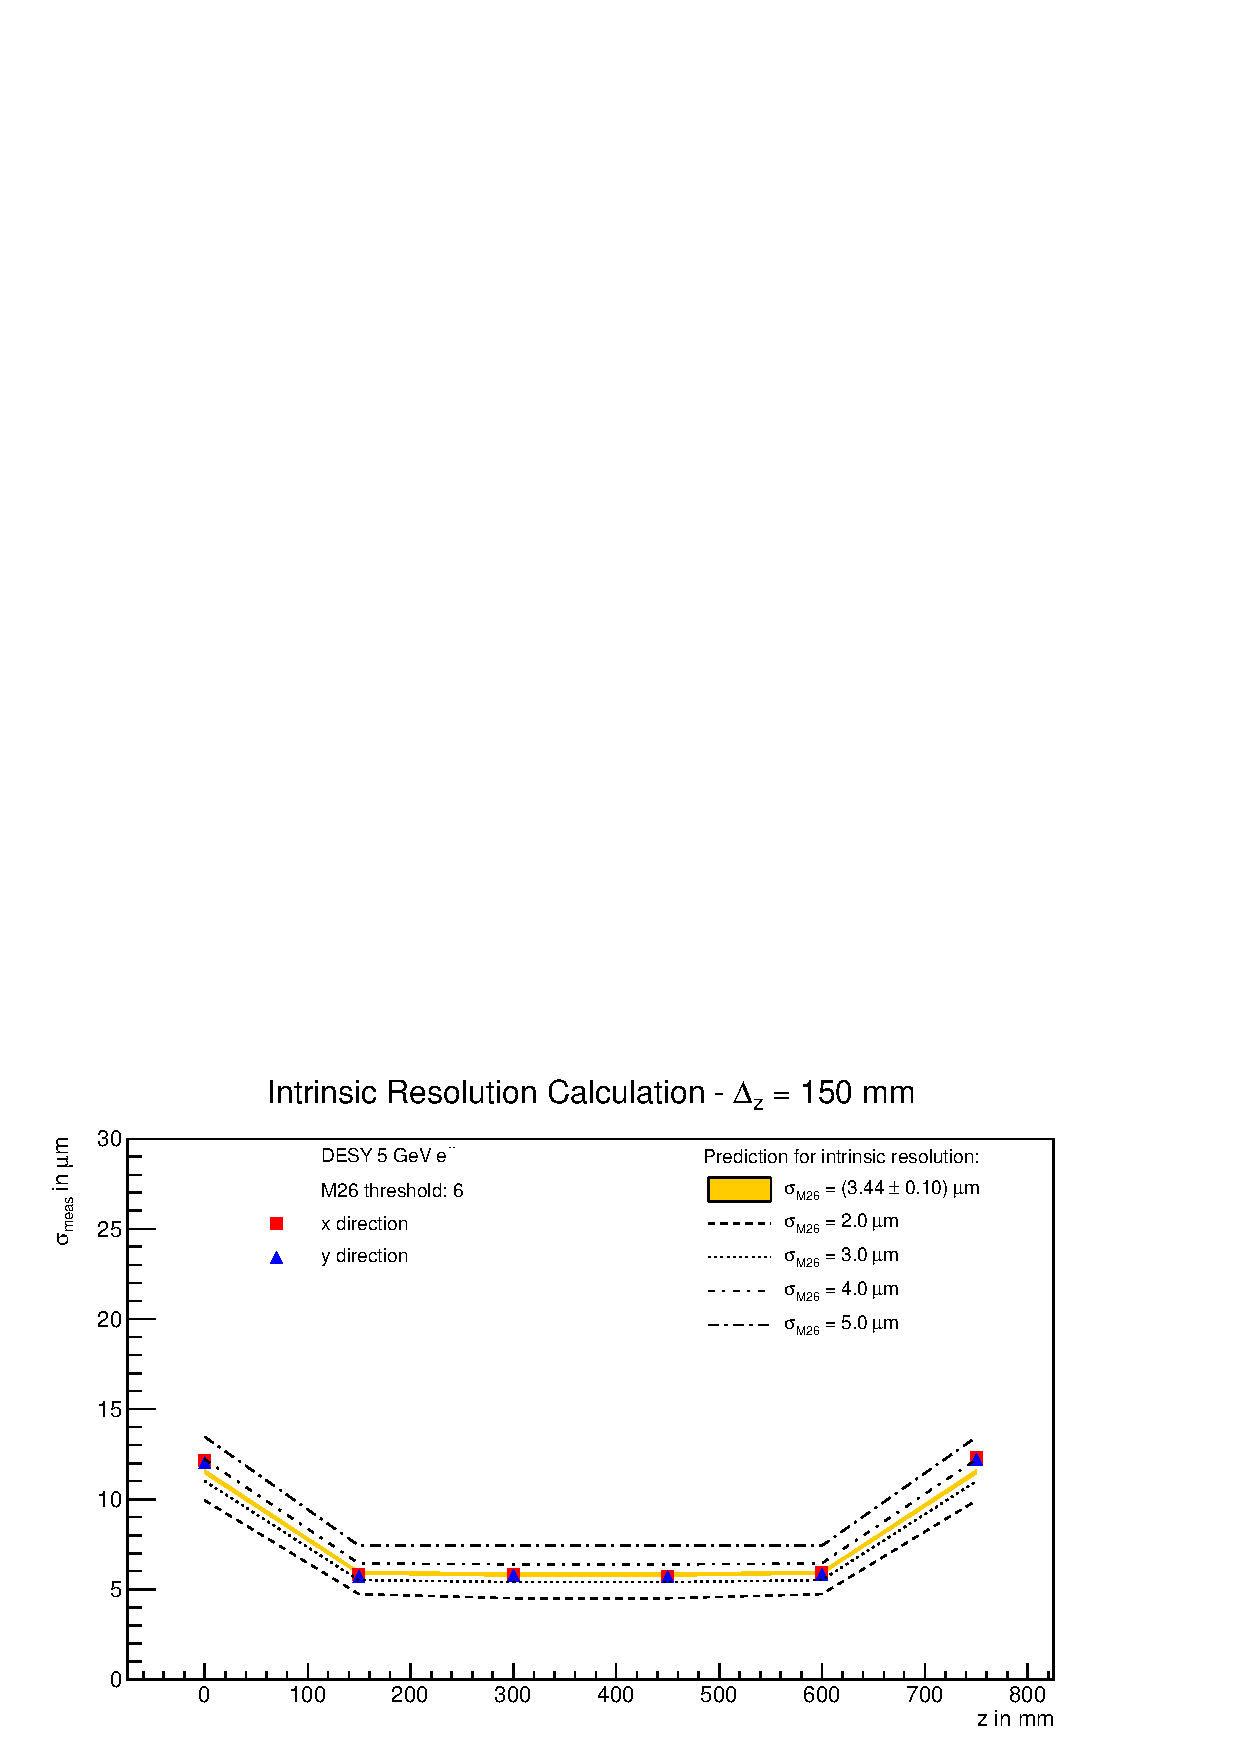
\includegraphics[width=\textwidth]{gfk/chapter03/wide_smiley.pdf}
\caption[Intrinsic telescope sensor resolution at $150\,\milli\meter$ plane
spacing]{Intrinsic telescope sensor resolution at $150\,\milli\meter$ plane
spacing.}
\label{fig:smileythick}
\end{figure}

In both cases, an error of $2.5\,\milli\meter$ on the plane distance
$\Delta_\textrm{z}$ was assumed. The predicted intrinsic resolution
$\sigma_{\textrm{M26}} = \sigma_{\textrm{Intrinsic}}$ of the MIMOSA 26 sensors
is \allowbreak$\left( 3.42\,\pm\, \allowbreak 0.12 \right)\,\micro\meter$ for a
plane spacing of
$20\,\milli\meter$, $\left( 3.44\,\pm\,0.10 \right)\,\micro\meter$ for a plane
spacing of $150\,\milli\meter$. For both geometries, the expected resolution of
$\approx\,3.5\,\micro\meter$, according to~\cite{ref:mimosa26}, can be
confirmed. The underlying assumptions in the method presented here are:\\

\begin{itemize}
\item The intrinsic resolution $\sigma_{\textrm{Intrinsic}}$ of all sensor
planes is assumed to be equal. As the discriminator thresholds are set for
subframes of each plane individually, however, this is not necessarily true.
Figure~\ref{fig:resivsenergy} shows the dependence of
$\sigma_{\textrm{Intrinsic}}$ on the applied threshold.\\

\item The multiple scattering term in
equation~\ref{eq:telescoperesolutionequation_2} is only calculated considering
the nominal sensor thicknesses, the air between sensor planes, and a
$25\,\micro\meter$ thick capton foil on either side of each sensor. The particle
momentum assumed is the nominal beam momentum.\\

\item Residuals are calculated using straight-line tracks only. Inclined tracks,
or a deflection of tracks in planes or scattering material, are not
considered.\\
\end{itemize}

\begin{figure}[hbtp]
\centering

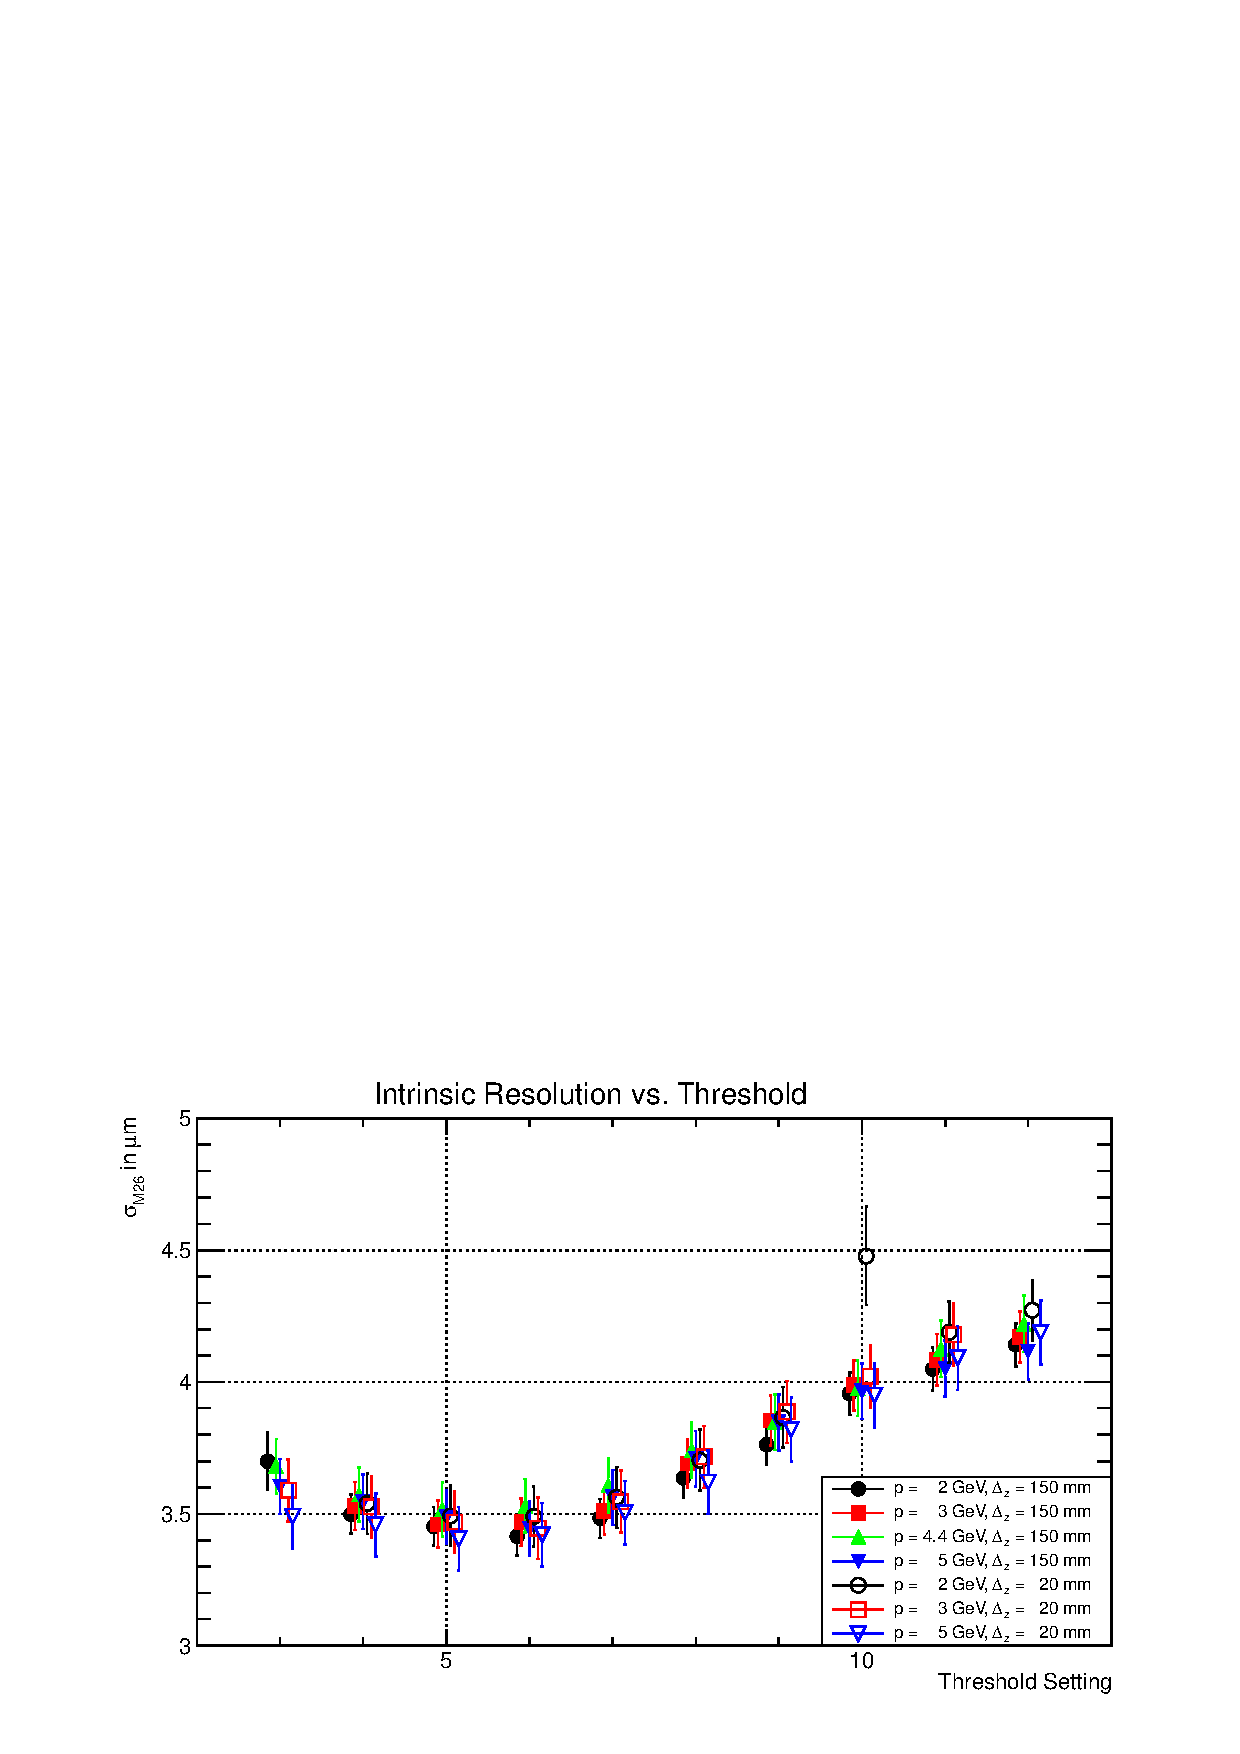
\includegraphics[width=\textwidth]{gfk/chapter03/resi_thresh_errors.pdf}
\caption[Telescope intrinsic sensor resolution for different threshold settings,
beam momenta and geometries]{The measured intrinsic resolution of the DATURA
telescope's MIMOSA 26 sensors $\sigma_{\textrm{M26}}$ for different beam momenta
p, sensor spacing $\Delta_{\textrm{z}}$ and applied sensor threshold. Some
values are shifted on the x-axis for improved legibility.}
\label{fig:resivsenergy}
\end{figure}

Figure~\ref{fig:resivsenergy} shows the calculated intrinsic telescope sensor
resolution for different beam energies, plane distances and applied sensor
thresholds. The minimum of the MIMOSA 26 sensors' intrinsic resolution is
reached for a threshold setting of $6$. While the measured residual width for
wider sensor spacings or lower beam momenta is higher, as can be seen in
figures~\ref{fig:smileythin} and~\ref{fig:smileythick}, these effects are
accounted for in equation~\ref{eq:telescoperesolutionequation} by the terms
$\sigma_{\textrm{Tel}}^2$ and $\sigma_{\textrm{MS}}^2$. Because of this, the
difference in intrinsic sensor resolution between configurations at any given
threshold is only approximately $\pm\,0.15\,\micro\meter$, which is well within
the errors.\\


Measurements by Behr~\cite{ref:j.behrmeasurements}, taken at high thresholds
$>\,10$ show comparable results of $\sigma_{\textrm{M26}} =
(4.35\,\pm\,0.10)\,\micro\meter$. Extrapolating to infinite energies, as
suggested in~\cite{ref:cmosbeamtest} and~\cite{ref:moritzthesis} by a fit over
the inverse square energy, to measure the intrinsic telescope sensor resolution
without multiple scattering effects, was not entirely successfull. This is in
parts due to the uncertainty of the beam energy, caused by deviations in the
dipole magnet current, as shown in~\cite{ref:summerstudentbrm}\\

The signal-to-noise threshold applied to each telescope sensor is a critical
parameter for a telescope's performance. A higher threshold will cut into the
signal, thus reducing the amount of clusters found on each plane and therefore
reducing the amount of reconstructable tracks. This reduces a sensor's
efficiency. A lower threshold will allow an increasing amount of noise hits to
be wrongly identified as clusters. This again will also lead to a broadening of
the residual distributions. Figure~\ref{fig:effi} shows the efficiency
distribution over a sensor plane. The efficiency is defined as the ratio of hits
being measured in the vicinity of a traversing track to the overall number of
tracks. $100\,\micro\meter$ was considered as maximum distance. A noisy pixel
column at $\approx Y = -8\,\milli\meter$ can be observed. This column was masked
during the converter step in the \texttt{datura-noDUT} example and subsequently
is not used during the analysis. Disregarding this area, an overall average
efficiency over $98\,\%$ is observed.\\

\begin{figure}[hbtp]
\centering
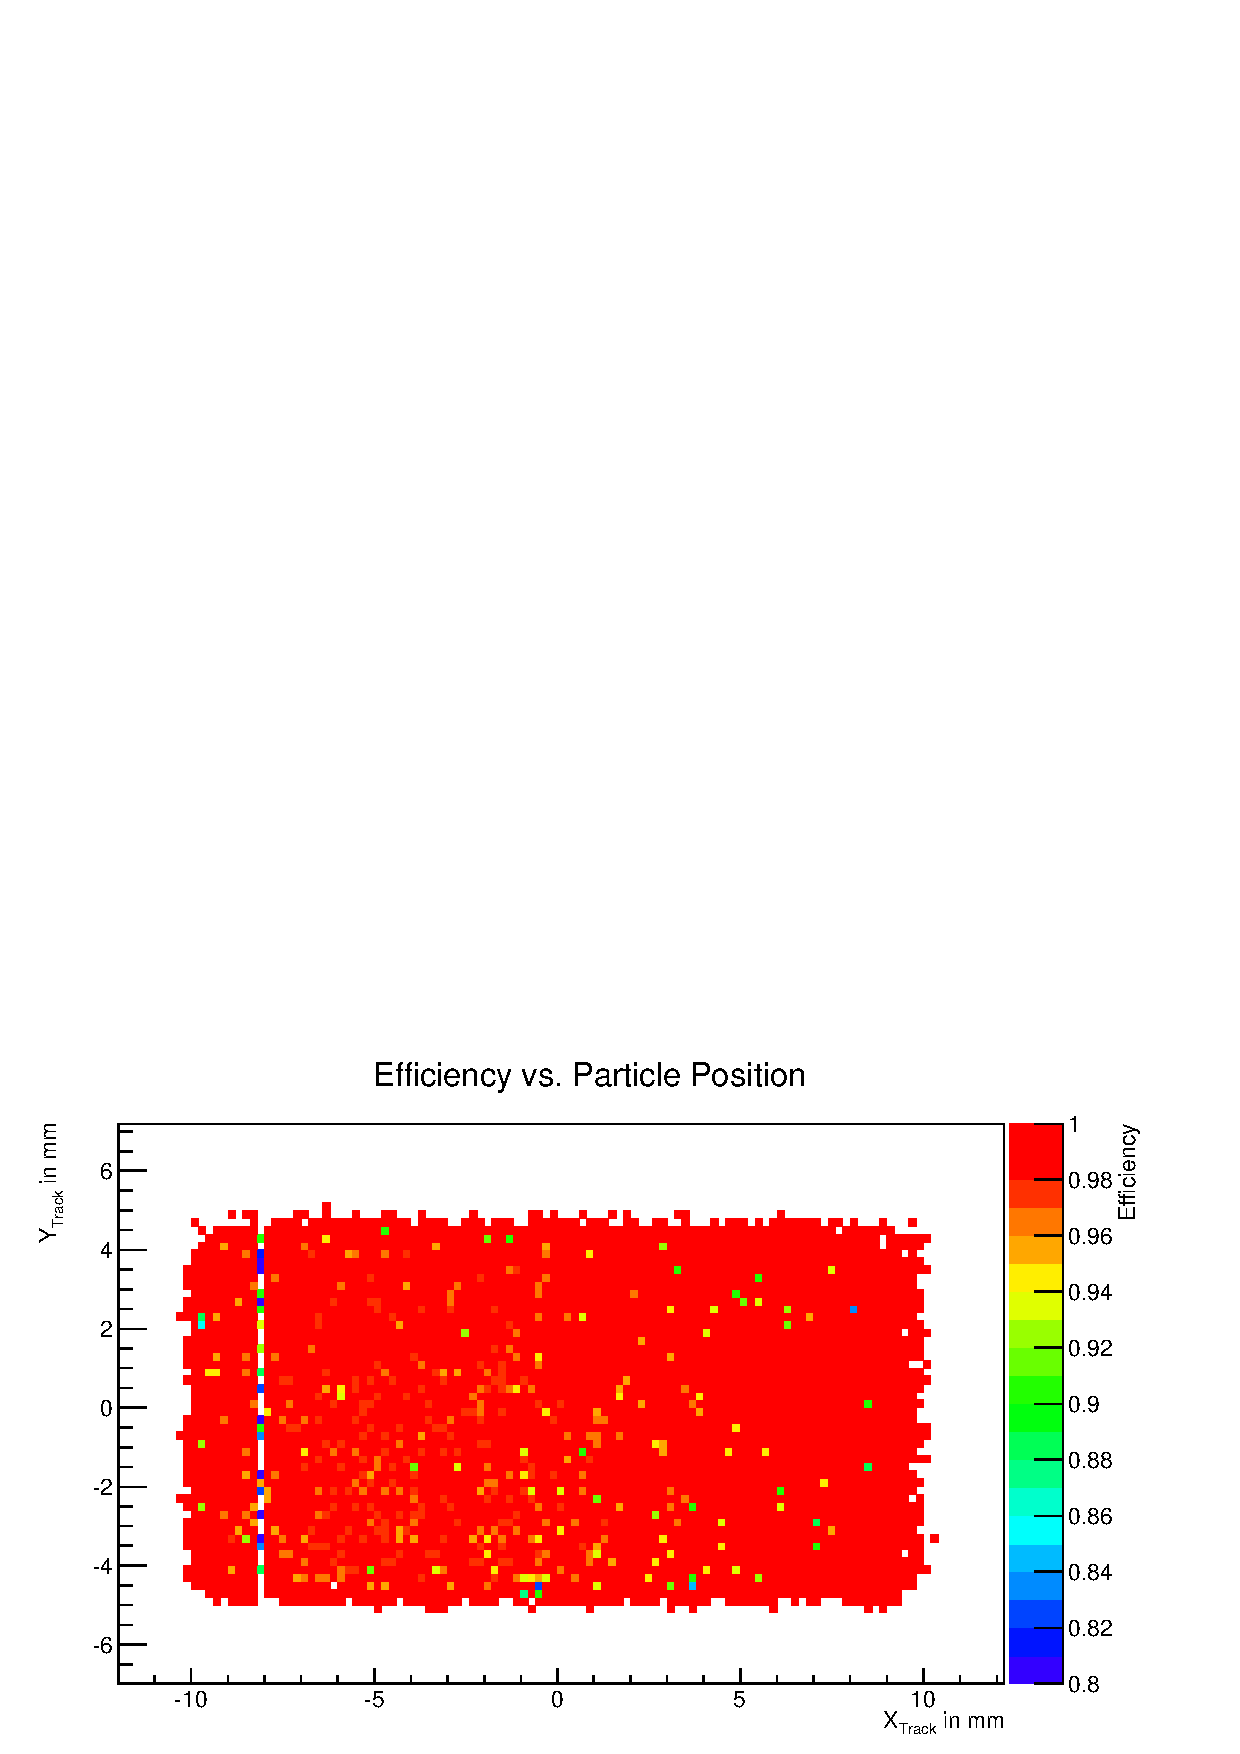
\includegraphics[width=\textwidth]{gfk/chapter03/plane3_effi_run37.pdf}
\caption[Telescope sensor efficiency]{Efficiency of telescope sensor plane $3$
at a threshold of $7$ and $5\,\giga\electronvolt$ beam momentum.}
\label{fig:effi}
\end{figure}

In figure~\ref{fig:effi_thresh}, the efficiency dependence on the sensor
threshold is shown, for various beam momenta and sensor spacings. Efficiencies
are averaged for all six sensor planes and both spatial coordinates. In all
cases, the efficiency is $\ge\,98\,\%$ up to a threshold setting of 7. With
increasing threshold, the efficiency declines, until an efficiency of $86\,\%$
for threshold $12$ is reached. The difference between momenta and plane spacings
is due to multiple scattering and increased telescope resolution.\\

\begin{figure}[hbtp]
\centering
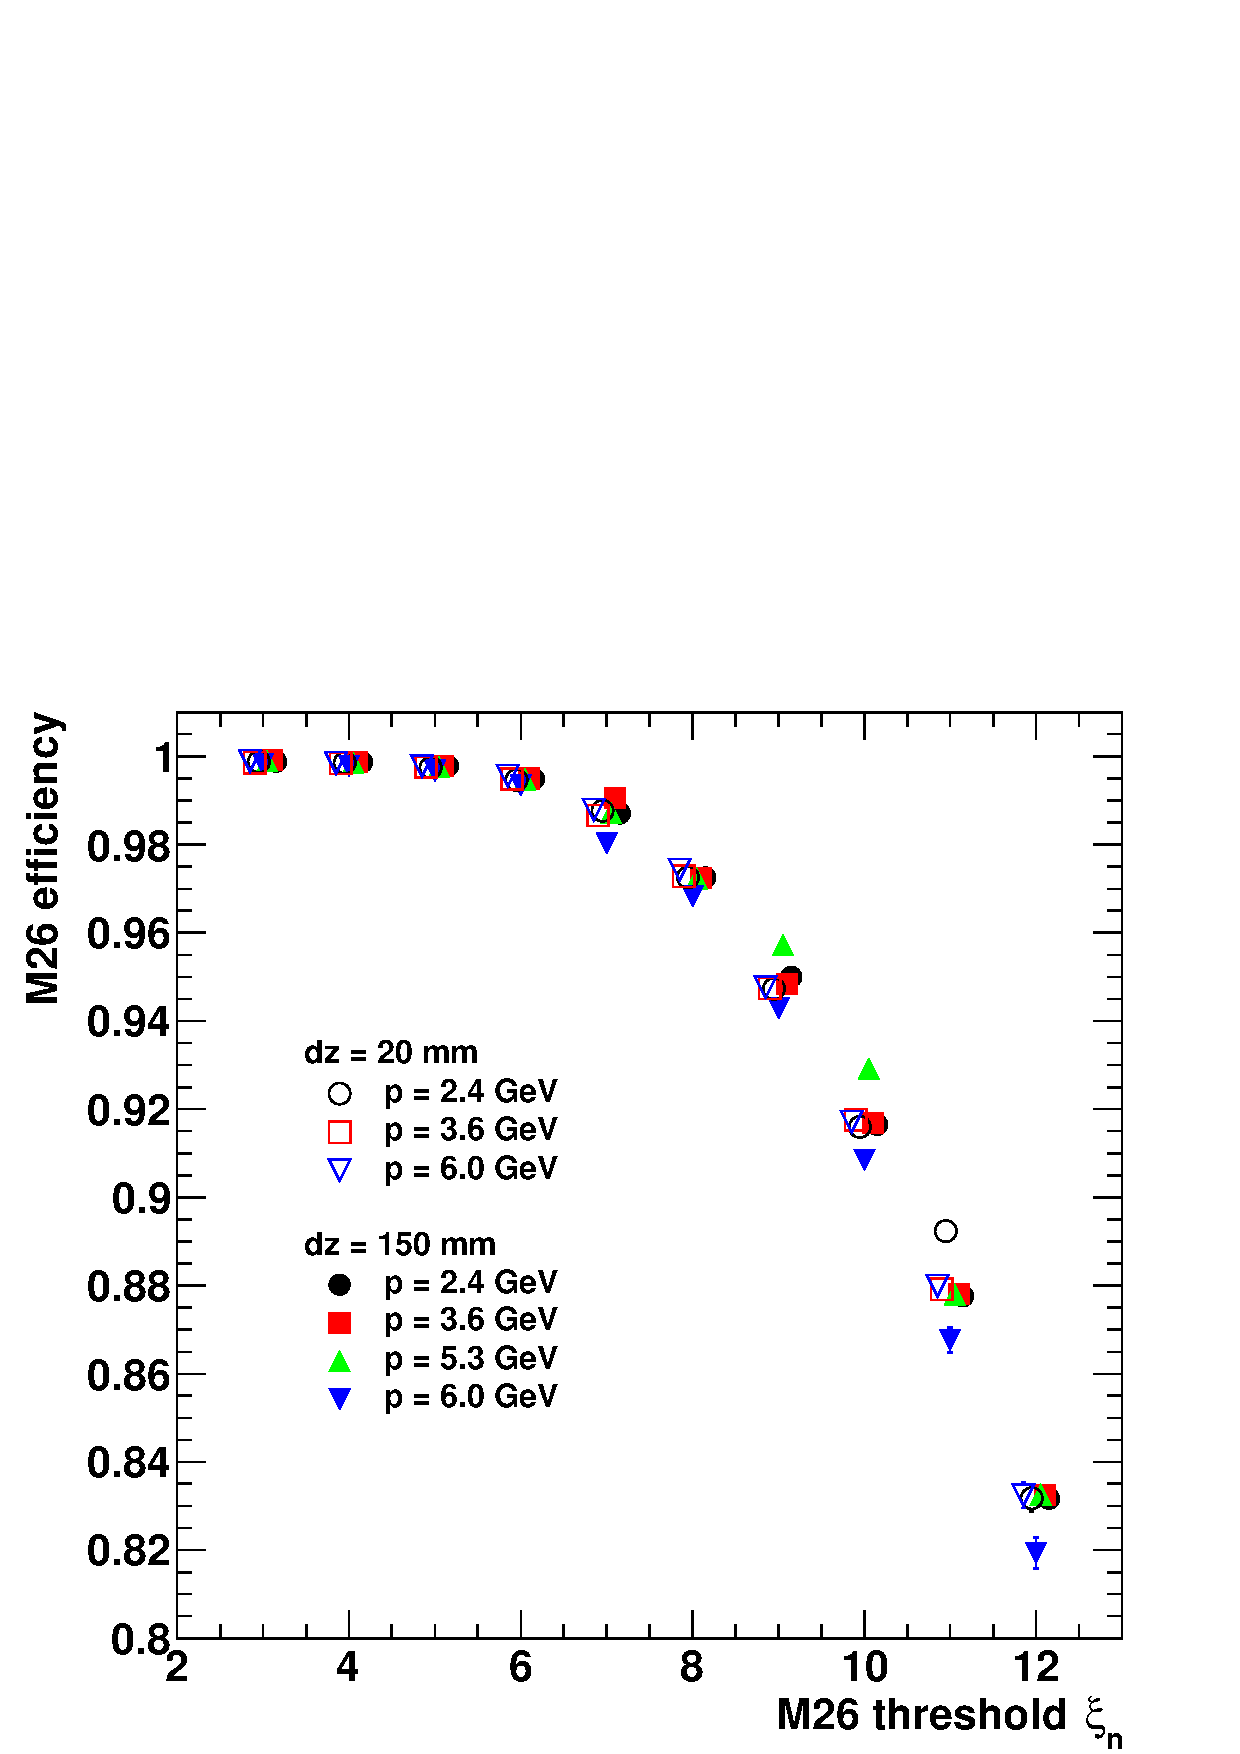
\includegraphics[width=\textwidth]{gfk/chapter03/effi_thresh.pdf}
\caption[Overall telescope sensor efficiency vs. threshold for different beam
momenta and sensor spacings]{Average efficiency of all telescope sensors in both
dimensions for different beam momenta and sensor spacing vs. applied threshold.
An efficiency decline with increasing threshold can be observed. Some values are
shifted on the x-axis for improved legibility.}
\label{fig:effi_thresh}
\end{figure}



\section{Conclusion}

\section*{Acknowledgement}

\small
\bibliographystyle{plain}
\bibliography{bibtex/refs}

\end{document}


